\documentclass[dvipsnames,table]{article}

% if you need to pass options to natbib, use, e.g.:
%     \PassOptionsToPackage{numbers, compress}{natbib}
% before loading neurips_data_2023

% ready for submission
\usepackage{neurips_data_2024}
\usepackage{listings}
\usepackage[table,dvipsnames]{xcolor}
\usepackage{aas_macros}
% to compile a preprint version, add the [preprint] option, e.g.:
%     \usepackage[preprint]{neurips_data_2023}
% This will indicate that the work is currently under review.

% to compile a camera-ready version, add the [final] option, e.g.:
%     \usepackage[final]{neurips_data_2023}

% to avoid loading the natbib package, add option nonatbib:
%    \usepackage[nonatbib]{neurips_data_2023}

% Submissions to the datasets and benchmarks are typically non anonymous,
% but anonymous submissions are allowed. If you feel that you must submit 
% anonymously, you can compile an anonymous version by adding the [anonymous] 
% option, e.g.:
%     \usepackage[anonymous]{neurips_data_2023}
% This will hide all author names.

\usepackage[utf8]{inputenc} % allow utf-8 input
\usepackage[T1]{fontenc}    % use 8-bit T1 fonts
\usepackage{hyperref}       % hyperlinks
\usepackage{url}            % simple URL typesetting
\usepackage{booktabs}       % professional-quality tables
\usepackage{amsfonts}       % blackboard math symbols
\usepackage{nicefrac}       % compact symbols for 1/2, etc.
\usepackage{microtype}      % microtypography
\usepackage{emoji}
\usepackage{amsmath}
\usepackage{threeparttable}
\usepackage{multirow}
\usepackage{colortbl}
\usepackage{cellspace}
\usepackage{xspace}
\usepackage{wrapfig}
\usepackage{array}
\usepackage{enumitem}

\setlength\aboverulesep{0pt}
\setlength\belowrulesep{0pt}

\hypersetup{
  colorlinks   = true, 
  urlcolor     = RoyalPurple, 
  linkcolor    = RoyalPurple,
  citecolor   = RoyalPurple 
}
\definecolor{verylightgray}{gray}{0.90} 

\definecolor{mygreen}{RGB}{226, 240, 217}
\definecolor{myblue}{RGB}{222, 235, 247}
\definecolor{myorange}{RGB}{251, 229, 214}
\definecolor{mygray}{RGB}{219, 219, 219}
\DeclareRobustCommand{\hlgreen}[1]{{\sethlcolor{mygreen}\hl{#1}}}
\DeclareRobustCommand{\hlblue}[1]{{\sethlcolor{myblue}\hl{#1}}}
\DeclareRobustCommand{\hlorange}[1]{{\sethlcolor{myorange}\hl{#1}}}
\DeclareRobustCommand{\hlgray}[1]{{\sethlcolor{mygray}\hl{#1}}}

\newcommand\pile{\textsc{Multimodal Universe}\xspace}

\newcommand{\FL}[1]{{\color{magenta}FL: #1}}
\newcommand{\MHC}[1]{{\color{red}MHC: #1}}
\newcommand{\LP}[1]{{\color{red}LP: #1}}
\newcommand{\HQ}[1]{{\color{red}HQ: #1}}
\newcommand{\RMG}[1]{{\color{red}RMG: #1}}
\newcommand{\MB}[1]{{\color{violet}MB: #1}}
\newcommand{\IC}[1]{{\color{blue}IC: #1}}
\newcommand{\SH}[1]{{\color{green}IC: #1}}
\newcommand{\MJS}[1]{{\color{orange}MJS: #1}}
\newcommand{\BCtwo}[1]{{\color{purple}BC: #1}}
\newcommand{\MDC}[1]{{\color{red}Miles: #1}}

\usepackage{tikz}
\usetikzlibrary{shapes.geometric, arrows.meta, positioning}

\tikzstyle{process} = [rectangle, rounded corners, minimum width=2cm, minimum height=1cm, text centered, draw=black, fill=blue!20]
\tikzstyle{arrow} = [thick,->,>=stealth]
\tikzstyle{data} = [cylinder, shape border rotate=90, draw, minimum height=1.5cm, minimum width=1cm, text centered, draw=black, fill=red!20]

%%% THIS FILE IS AUTOMATICALLY GENERATED.  DON'T MODIFY, OR YOUR CHANGES MIGHT BE OVERWRITTEN!
\newcommand\poi{\ensuremath{\text{Poi}}}
\newcommand\est[1]{\bs{\hat \mu_{#1}}}
\newcommand\true{\ensuremath{\bs{\mu^\star}}}
\newcommand\sa{\ensuremath{\mathcal{a}}}
\newcommand\sd{\ensuremath{\mathcal{d}}}
\newcommand\se{\ensuremath{\mathcal{e}}}
\newcommand\sg{\ensuremath{\mathcal{g}}}
\newcommand\sh{\ensuremath{\mathcal{h}}}
\newcommand\si{\ensuremath{\mathcal{i}}}
\newcommand\sj{\ensuremath{\mathcal{j}}}
\newcommand\sk{\ensuremath{\mathcal{k}}}
\newcommand\sm{\ensuremath{\mathcal{m}}}
\newcommand\sn{\ensuremath{\mathcal{n}}}
\newcommand\so{\ensuremath{\mathcal{o}}}
\newcommand\sq{\ensuremath{\mathcal{q}}}
\newcommand\sr{\ensuremath{\mathcal{r}}}
\newcommand\st{\ensuremath{\mathcal{t}}}
\newcommand\su{\ensuremath{\mathcal{u}}}
\newcommand\sv{\ensuremath{\mathcal{v}}}
\newcommand\sw{\ensuremath{\mathcal{w}}}
\newcommand\sx{\ensuremath{\mathcal{x}}}
\newcommand\sy{\ensuremath{\mathcal{y}}}
\newcommand\sz{\ensuremath{\mathcal{z}}}
\newcommand\sA{\ensuremath{\mathcal{A}}}
\newcommand\sB{\ensuremath{\mathcal{B}}}
\newcommand\sC{\ensuremath{\mathcal{C}}}
\newcommand\sD{\ensuremath{\mathcal{D}}}
\newcommand\sE{\ensuremath{\mathcal{E}}}
\newcommand\sF{\ensuremath{\mathcal{F}}}
\newcommand\sG{\ensuremath{\mathcal{G}}}
\newcommand\sH{\ensuremath{\mathcal{H}}}
\newcommand\sI{\ensuremath{\mathcal{I}}}
\newcommand\sJ{\ensuremath{\mathcal{J}}}
\newcommand\sK{\ensuremath{\mathcal{K}}}
\newcommand\sL{\ensuremath{\mathcal{L}}}
\newcommand\sM{\ensuremath{\mathcal{M}}}
\newcommand\sN{\ensuremath{\mathcal{N}}}
\newcommand\sO{\ensuremath{\mathcal{O}}}
\newcommand\sP{\ensuremath{\mathcal{P}}}
\newcommand\sQ{\ensuremath{\mathcal{Q}}}
\newcommand\sR{\ensuremath{\mathcal{R}}}
\newcommand\sS{\ensuremath{\mathcal{S}}}
\newcommand\sT{\ensuremath{\mathcal{T}}}
\newcommand\sU{\ensuremath{\mathcal{U}}}
\newcommand\sV{\ensuremath{\mathcal{V}}}
\newcommand\sW{\ensuremath{\mathcal{W}}}
\newcommand\sX{\ensuremath{\mathcal{X}}}
\newcommand\sY{\ensuremath{\mathcal{Y}}}
\newcommand\sZ{\ensuremath{\mathcal{Z}}}
\newcommand\ba{\ensuremath{\mathbf{a}}}
\newcommand\bb{\ensuremath{\mathbf{b}}}
\newcommand\bc{\ensuremath{\mathbf{c}}}
\newcommand\bd{\ensuremath{\mathbf{d}}}
\newcommand\be{\ensuremath{\mathbf{e}}}
\newcommand\bg{\ensuremath{\mathbf{g}}}
\newcommand\bh{\ensuremath{\mathbf{h}}}
\newcommand\bi{\ensuremath{\mathbf{i}}}
\newcommand\bj{\ensuremath{\mathbf{j}}}
\newcommand\bk{\ensuremath{\mathbf{k}}}
\newcommand\bl{\ensuremath{\mathbf{l}}}
\newcommand\bn{\ensuremath{\mathbf{n}}}
\newcommand\bo{\ensuremath{\mathbf{o}}}
\newcommand\bp{\ensuremath{\mathbf{p}}}
\newcommand\bq{\ensuremath{\mathbf{q}}}
\newcommand\br{\ensuremath{\mathbf{r}}}
\newcommand\bs{\ensuremath{\boldsymbol}}
\newcommand\bt{\ensuremath{\mathbf{t}}}
\newcommand\bu{\ensuremath{\mathbf{u}}}
\newcommand\bv{\ensuremath{\mathbf{v}}}
\newcommand\bw{\ensuremath{\mathbf{w}}}
\newcommand\bx{\ensuremath{\mathbf{x}}}
\newcommand\by{\ensuremath{\mathbf{y}}}
\newcommand\bz{\ensuremath{\mathbf{z}}}
\newcommand\bA{\ensuremath{\mathbf{A}}}
\newcommand\bB{\ensuremath{\mathbf{B}}}
\newcommand\bC{\ensuremath{\mathbf{C}}}
\newcommand\bD{\ensuremath{\mathbf{D}}}
\newcommand\bE{\ensuremath{\mathbf{E}}}
\newcommand\bF{\ensuremath{\mathbf{F}}}
\newcommand\bG{\ensuremath{\mathbf{G}}}
\newcommand\bH{\ensuremath{\mathbf{H}}}
\newcommand\bI{\ensuremath{\mathbf{I}}}
\newcommand\bJ{\ensuremath{\mathbf{J}}}
\newcommand\bK{\ensuremath{\mathbf{K}}}
\newcommand\bL{\ensuremath{\mathbf{L}}}
\newcommand\bM{\ensuremath{\mathbf{M}}}
\newcommand\bN{\ensuremath{\mathbf{N}}}
\newcommand\bO{\ensuremath{\mathbf{O}}}
\newcommand\bP{\ensuremath{\mathbf{P}}}
\newcommand\bQ{\ensuremath{\mathbf{Q}}}
\newcommand\bR{\ensuremath{\mathbf{R}}}
\newcommand\bS{\ensuremath{\mathbf{S}}}
\newcommand\bT{\ensuremath{\mathbf{T}}}
\newcommand\bU{\ensuremath{\mathbf{U}}}
\newcommand\bV{\ensuremath{\mathbf{V}}}
\newcommand\bW{\ensuremath{\mathbf{W}}}
\newcommand\bX{\ensuremath{\mathbf{X}}}
\newcommand\bY{\ensuremath{\mathbf{Y}}}
\newcommand\bZ{\ensuremath{\mathbf{Z}}}
\newcommand\Ba{\ensuremath{\mathbb{a}}}
\newcommand\Bb{\ensuremath{\mathbb{b}}}
\newcommand\Bc{\ensuremath{\mathbb{c}}}
\newcommand\Bd{\ensuremath{\mathbb{d}}}
\newcommand\Be{\ensuremath{\mathbb{e}}}
\newcommand\Bf{\ensuremath{\mathbb{f}}}
\newcommand\Bg{\ensuremath{\mathbb{g}}}
\newcommand\Bh{\ensuremath{\mathbb{h}}}
\newcommand\Bi{\ensuremath{\mathbb{i}}}
\newcommand\Bj{\ensuremath{\mathbb{j}}}
\newcommand\Bk{\ensuremath{\mathbb{k}}}
\newcommand\Bl{\ensuremath{\mathbb{l}}}
\newcommand\Bm{\ensuremath{\mathbb{m}}}
\newcommand\Bn{\ensuremath{\mathbb{n}}}
\newcommand\Bo{\ensuremath{\mathbb{o}}}
\newcommand\Bp{\ensuremath{\mathbb{p}}}
\newcommand\Bq{\ensuremath{\mathbb{q}}}
\newcommand\Br{\ensuremath{\mathbb{r}}}
\newcommand\Bs{\ensuremath{\mathbb{s}}}
\newcommand\Bt{\ensuremath{\mathbb{t}}}
\newcommand\Bu{\ensuremath{\mathbb{u}}}
\newcommand\Bv{\ensuremath{\mathbb{v}}}
\newcommand\Bw{\ensuremath{\mathbb{w}}}
\newcommand\Bx{\ensuremath{\mathbb{x}}}
\newcommand\By{\ensuremath{\mathbb{y}}}
\newcommand\Bz{\ensuremath{\mathbb{z}}}
\newcommand\BA{\ensuremath{\mathbb{A}}}
\newcommand\BB{\ensuremath{\mathbb{B}}}
\newcommand\BC{\ensuremath{\mathbb{C}}}
\newcommand\BD{\ensuremath{\mathbb{D}}}
\newcommand\BE{\ensuremath{\mathbb{E}}}
\newcommand\BF{\ensuremath{\mathbb{F}}}
\newcommand\BG{\ensuremath{\mathbb{G}}}
\newcommand\BH{\ensuremath{\mathbb{H}}}
\newcommand\BI{\ensuremath{\mathbb{I}}}
\newcommand\BJ{\ensuremath{\mathbb{J}}}
\newcommand\BK{\ensuremath{\mathbb{K}}}
\newcommand\BL{\ensuremath{\mathbb{L}}}
\newcommand\BM{\ensuremath{\mathbb{M}}}
\newcommand\BN{\ensuremath{\mathbb{N}}}
\newcommand\BO{\ensuremath{\mathbb{O}}}
\newcommand\BP{\ensuremath{\mathbb{P}}}
\newcommand\BQ{\ensuremath{\mathbb{Q}}}
\newcommand\BR{\ensuremath{\mathbb{R}}}
\newcommand\BS{\ensuremath{\mathbb{S}}}
\newcommand\BT{\ensuremath{\mathbb{T}}}
\newcommand\BU{\ensuremath{\mathbb{U}}}
\newcommand\BV{\ensuremath{\mathbb{V}}}
\newcommand\BW{\ensuremath{\mathbb{W}}}
\newcommand\BX{\ensuremath{\mathbb{X}}}
\newcommand\BY{\ensuremath{\mathbb{Y}}}
\newcommand\BZ{\ensuremath{\mathbb{Z}}}
\newcommand\balpha{\ensuremath{\mbox{\boldmath$\alpha$}}}
\newcommand\bbeta{\ensuremath{\mbox{\boldmath$\beta$}}}
\newcommand\btheta{\ensuremath{\mbox{\boldmath$\theta$}}}
\newcommand\bphi{\ensuremath{\mbox{\boldmath$\phi$}}}
\newcommand\bpi{\ensuremath{\mbox{\boldmath$\pi$}}}
\newcommand\bpsi{\ensuremath{\mbox{\boldmath$\psi$}}}
\newcommand\bmu{\ensuremath{\mbox{\boldmath$\mu$}}}

% Figures
\newcommand\fig[1]{\begin{center} \includegraphics{#1} \end{center}}
\newcommand\Fig[4]{\begin{figure}[ht] \begin{center} \includegraphics[scale=#2]{#1} \end{center} \vspace{-1.0em} \caption{\label{fig:#3} #4} \vspace{-.5em} \end{figure}}
\newcommand\FigTop[4]{\begin{figure}[t] \begin{center} \includegraphics[scale=#2]{#1} \end{center} \vspace{-1.0em} \caption{\label{fig:#3} #4} \vspace{-.5em} \end{figure}}
\newcommand\FigStar[4]{\begin{figure*}[ht] \begin{center} \includegraphics[scale=#2]{#1} \end{center} \caption{\label{fig:#3} #4} \end{figure*}}
\newcommand\FigRight[4]{\begin{wrapfigure}{r}{0.5\textwidth} \begin{center} \includegraphics[width=0.5\textwidth]{#1} \end{center} \caption{\label{fig:#3} #4} \end{wrapfigure}}
\newcommand\aside[1]{\quad\text{[#1]}}
\newcommand\interpret[1]{\llbracket #1 \rrbracket} % Denotation
% operators
\DeclareMathOperator*{\tr}{tr}
\DeclareMathOperator*{\sign}{sign}
\newcommand{\var}{\text{Var}} % Variance
\DeclareMathOperator*{\cov}{Cov} % Covariance
\DeclareMathOperator*{\diag}{diag} % Diagonal matrix
\newcommand\p[1]{\ensuremath{\left( #1 \right)}} % Parenthesis ()
\newcommand\pa[1]{\ensuremath{\left\langle #1 \right\rangle}} % <>
\newcommand\pb[1]{\ensuremath{\left[ #1 \right]}} % []
\newcommand\pc[1]{\ensuremath{\left\{ #1 \right\}}} % {}
\newcommand\eval[2]{\ensuremath{\left. #1 \right|_{#2}}} % Integral evaluation
\newcommand\inv[1]{\ensuremath{\frac{1}{#1}}}
\newcommand\half{\ensuremath{\frac{1}{2}}}
\newcommand\R{\ensuremath{\mathbb{R}}} % Real numbers
\newcommand\Z{\ensuremath{\mathbb{Z}}} % Integers
\newcommand\inner[2]{\ensuremath{\left< #1, #2 \right>}} % Inner product
\newcommand\mat[2]{\ensuremath{\left(\begin{array}{#1}#2\end{array}\right)}} % Matrix
\newcommand\eqn[1]{\begin{align} #1 \end{align}} % Equation (array)
\newcommand\eqnl[2]{\begin{align} \label{eqn:#1} #2 \end{align}} % Equation (array) with label
\newcommand\eqdef{\ensuremath{\stackrel{\rm def}{=}}} % Equal by definition
\newcommand{\1}{\mathbb{I}} % Indicator (don't use \mathbbm{1} because bbm is not TrueType)
\newcommand{\bone}{\mathbf{1}} % for vector one
\newcommand{\bzero}{\mathbf{0}} % for vector zero
\newcommand\refeqn[1]{(\ref{eqn:#1})}
\newcommand\refeqns[2]{(\ref{eqn:#1}) and (\ref{eqn:#2})}
\newcommand\refchp[1]{Chapter~\ref{chp:#1}}
\newcommand\refsec[1]{Section~\ref{sec:#1}}
\newcommand\refsecs[2]{Sections~\ref{sec:#1} and~\ref{sec:#2}}
\newcommand\reffig[1]{Figure~\ref{fig:#1}}
\newcommand\reffigs[2]{Figures~\ref{fig:#1} and~\ref{fig:#2}}
\newcommand\reffigss[3]{Figures~\ref{fig:#1},~\ref{fig:#2}, and~\ref{fig:#3}}
\newcommand\reffigsss[4]{Figures~\ref{fig:#1},~\ref{fig:#2},~\ref{fig:#3}, and~\ref{fig:#4}}
\newcommand\reftab[1]{Table~\ref{tab:#1}}
\newcommand\refapp[1]{Appendix~\ref{sec:#1}}
\newcommand\refthm[1]{Theorem~\ref{thm:#1}}
\newcommand\refthms[2]{Theorems~\ref{thm:#1} and~\ref{thm:#2}}
\newcommand\reflem[1]{Lemma~\ref{lem:#1}}
\newcommand\reflems[2]{Lemmas~\ref{lem:#1} and~\ref{lem:#2}}
\newcommand\refalg[1]{Algorithm~\ref{alg:#1}}
\newcommand\refalgs[2]{Algorithms~\ref{alg:#1} and~\ref{alg:#2}}
\newcommand\refex[1]{Example~\ref{ex:#1}}
\newcommand\refexs[2]{Examples~\ref{ex:#1} and~\ref{ex:#2}}
\newcommand\refprop[1]{Proposition~\ref{prop:#1}}
\newcommand\refdef[1]{Definition~\ref{def:#1}}
\newcommand\refcor[1]{Corollary~\ref{cor:#1}}
\newcommand\Chapter[2]{\chapter{#2}\label{chp:#1}}
\newcommand\Section[2]{\section{#2}\label{sec:#1}}
\newcommand\Subsection[2]{\subsection{#2}\label{sec:#1}}
\newcommand\Subsubsection[2]{\subsubsection{#2}\label{sec:#1}}
\ifthenelse{\isundefined{\definition}}{\newtheorem{definition}{Definition}}{}
\ifthenelse{\isundefined{\assumption}}{\newtheorem{assumption}{Assumption}}{}
\ifthenelse{\isundefined{\hypothesis}}{\newtheorem{hypothesis}{Hypothesis}}{}
\ifthenelse{\isundefined{\proposition}}{\newtheorem{proposition}{Proposition}}{}
\ifthenelse{\isundefined{\theorem}}{\newtheorem{theorem}{Theorem}}{}
\ifthenelse{\isundefined{\lemma}}{\newtheorem{lemma}{Lemma}}{}
\ifthenelse{\isundefined{\corollary}}{\newtheorem{corollary}{Corollary}}{}
\ifthenelse{\isundefined{\alg}}{\newtheorem{alg}{Algorithm}}{}
\ifthenelse{\isundefined{\example}}{\newtheorem{example}{Example}}{}
\newcommand\cv{\ensuremath{\to}} % Convergence
\newcommand\cvL{\ensuremath{\xrightarrow{\mathcal{L}}}} % Convergence in law
\newcommand\cvd{\ensuremath{\xrightarrow{d}}} % Convergence in distribution
\newcommand\cvP{\ensuremath{\xrightarrow{P}}} % Convergence in probability
\newcommand\cvas{\ensuremath{\xrightarrow{a.s.}}} % Convergence almost surely
\newcommand\eqdistrib{\ensuremath{\stackrel{d}{=}}} % Equal in distribution
\newcommand{\E}{\ensuremath{\mathbb{E}}} % Expectation
\newcommand\KL[2]{\ensuremath{\text{KL}\left( #1 \| #2 \right)}} % KL-divergence

\usepackage{bm}
% Vectors
\def\vzero{{\bm{0}}}
\def\vone{{\bm{1}}}
\def\vmu{{\bm{\mu}}}
\def\vtheta{{\bm{\theta}}}
\def\va{{\bm{a}}}
\def\vb{{\bm{b}}}
\def\vc{{\bm{c}}}
\def\vd{{\bm{d}}}
\def\ve{{\bm{e}}}
\def\vf{{\bm{f}}}
\def\vg{{\bm{g}}}
\def\vh{{\bm{h}}}
\def\vi{{\bm{i}}}
\def\vj{{\bm{j}}}
\def\vk{{\bm{k}}}
\def\vl{{\bm{l}}}
\def\vm{{\bm{m}}}
\def\vn{{\bm{n}}}
\def\vo{{\bm{o}}}
\def\vp{{\bm{p}}}
\def\vq{{\bm{q}}}
\def\vr{{\bm{r}}}
\def\vs{{\bm{s}}}
\def\vt{{\bm{t}}}
\def\vu{{\bm{u}}}
\def\vv{{\bm{v}}}
\def\vw{{\bm{w}}}
\def\vx{{\bm{x}}}
\def\vy{{\bm{y}}}
\def\vz{{\bm{z}}}


% Matrix
\def\mA{{\bm{A}}}
\def\mB{{\bm{B}}}
\def\mC{{\bm{C}}}
\def\mD{{\bm{D}}}
\def\mE{{\bm{E}}}
\def\mF{{\bm{F}}}
\def\mG{{\bm{G}}}
\def\mH{{\bm{H}}}
\def\mI{{\bm{I}}}
\def\mJ{{\bm{J}}}
\def\mK{{\bm{K}}}
\def\mL{{\bm{L}}}
\def\mM{{\bm{M}}}
\def\mN{{\bm{N}}}
\def\mO{{\bm{O}}}
\def\mP{{\bm{P}}}
\def\mQ{{\bm{Q}}}
\def\mR{{\bm{R}}}
\def\mS{{\bm{S}}}
\def\mT{{\bm{T}}}
\def\mU{{\bm{U}}}
\def\mV{{\bm{V}}}
\def\mW{{\bm{W}}}
\def\mX{{\bm{X}}}
\def\mY{{\bm{Y}}}
\def\mZ{{\bm{Z}}}
\def\mBeta{{\bm{\beta}}}
\def\mPhi{{\bm{\Phi}}}
\def\mLambda{{\bm{\Lambda}}}
\def\mSigma{{\bm{\Sigma}}}



\newtheorem{remark}{Remark}
\newtheorem{cor}{Corollary}
\newtheorem{condition}{Condition}
\newcommand{\loss}{\ell}
\newcommand{\losstext}{\text{loss}}
\newcommand{\pstar}{p^*}
\newcommand{\thetapre}{\theta_{\text{pre}}}

\newcommand{\classification}{\textsc{AstroClassification}\xspace}
\newcommand{\redshifts}{\textsc{Redshifts}\xspace}
\newcommand{\iwildcam}{\textsc{iWildCam-WILDS}\xspace}
\newcommand{\camelyon}{\textsc{Camelyon17-WILDS}\xspace}
\newcommand{\sft}{standard fine-tuning\xspace}
\newcommand{\Sft}{Standard fine-tuning\xspace}

% Misc. macros
\newcommand{\set}[1]{\left\{#1\right\}}
\newcommand{\absolute}[1]{|#1|}
\newcommand{\strongaugs}{strong-augs}

% Data macros
\newcommand{\augX}{\mX'}
\newcommand{\augXerr}{\mX'_{\text{err}}}
\newcommand{\Xin}{\mX}
\newcommand{\Xinerr}{\mX_{\text{err}}}
\newcommand{\znew}{z'}
\newcommand{\zorig}{z_{\text{orig}}}

\newcommand{\sourcedist}{P_S}
\newcommand{\targetdist}{P_T}
\newcommand{\unlabeldist}{P_U}
\newcommand{\sourcex}{\sX_\sS}
\newcommand{\targetx}{\sX_\sT}
\newcommand{\cdx}{\sX_{cd}}
\newcommand{\cdxsingle}{\inputx_{cd}}
\newcommand{\cdxo}[2]{\sX_{#1#2}} % class-domain pair with options
\newcommand{\cdxosingle}[2]{\inputx_{#1#2}}
\newcommand{\inputx}{x}
\newcommand{\labelvar}{y}
\newcommand{\labelx}{y_x}
\newcommand{\inputxp}{{x'}}
\newcommand{\labelxp}{y_{x'}}
\newcommand{\domainvar}{d}
\newcommand{\domainx}{d_x}
\newcommand{\domainxp}{d_{x'}}
\newcommand{\numcls}{r}
\newcommand{\numdom}{m}
\newcommand{\embeddim}{k}
\newcommand{\xsize}{N}
\newcommand{\cdsize}{n}
\newcommand{\posx}{\inputx^+}
\newcommand{\pospairdist}{S_+}
\newcommand{\dattract}{d_+}
\newcommand{\drepel}{d_-}

\newcommand{\inputspace}{\sX}
\newcommand{\labelspace}{\sY}
\newcommand{\repspace}{\sZ}
\newcommand{\aug}{\mathcal{A}_{\text{pre}}}
\newcommand{\augft}{\mathcal{A}_{\text{ft}}}
\newcommand{\augspace}{\mathcal{X}}
\newcommand{\augpoint}{x}
\newcommand{\natspace}{\overline{\mathcal{X}}}
\newcommand{\natpoint}{\overline{x}}
\DeclareMathOperator{\conn}{conn}
\newcommand{\Prob}[1]{\mathbb{P}\left[#1\right]}
\newcommand{\Probs}[2]{\mathbb{P}_{#1}\left[#2\right]}

\newcommand{\augproba}{{\alpha'}}
\newcommand{\augprobb}{{\beta'}}
\newcommand{\augprobg}{{\gamma'}}
\newcommand{\augprobr}{{\rho'}}

\newcommand{\pairproba}{{\alpha}}
\newcommand{\pairprobb}{{\beta}}
\newcommand{\pairprobg}{{\gamma}}
\newcommand{\pairprobr}{{\rho}}
\newcommand{\pairnorm}{{C}}

\newcommand{\posclass}{1}
\newcommand{\negclass}{-1}

\newcommand{\sbmg}{G}
\newcommand{\sbmv}{V}
\newcommand{\sbme}{E}

\newcommand{\losspre}{\losstext_{\text{pretrain}}}
\newcommand{\lossft}{\losstext_{\text{ft}}}

% Modeling macros
\newcommand{\encoder}{\phi}
\newcommand{\empencoder}{\widehat{\encoder}}
\newcommand{\empencoderMatrix}{\widehat{\Phi}}
\newcommand{\empencoderdann}{\widehat{\encoder}_\text{dann}}
\newcommand{\head}{h}
\newcommand{\dhead}{{\head}_{\text{dom}}}
\newcommand{\emphead}{\widehat{\head}}
\newcommand{\empheaddann}{\widehat{\head}_\text{dann}}
\newcommand{\clf}{f}
\newcommand{\empclf}{\widehat{\clf}}
\newcommand{\linmat}{B}
\newcommand{\emplinmat}{\widehat{\linmat}}
\newcommand{\empclferm}{\widehat{\clf}_\text{erm}}
\newcommand{\empclfdann}{\widehat{\clf}_\text{dann}}
\newcommand{\domainclf}{\dhead}
\newcommand{\domainclffam}{\sH_d}

% Objective
\newcommand{\lpretrain}{\sL_\text{pretrain}}
\newcommand{\ellpretrain}{\ell_\text{pretrain}}
\newcommand{\lfinetune}{\sL}
\newcommand{\ellfinetune}{\ell}
\newcommand{\elldomain}{\ell_d}
\newcommand{\batch}{M}
\newcommand{\auggraph}{G}
\newcommand{\Lzeroone}{\sL_{0-1}}
\newcommand{\Lerm}{\sL_\text{ERM}}
\newcommand{\Ldann}{\sL_\text{DANN}}
\newcommand{\LDzeroone}{\sL^{D}_{0-1}}


\newcommand{\lambdamax}{\lambda_{\text{max}}}
\newcommand{\onehot}{\text{one-hot}}
\newcommand{\lambdamin}{\lambda_{\text{min}}}
\newcommand{\fisherinfj}{I_{j,\thetastar}}
\newcommand{\fisherinfk}{I_{k,\thetastar}}
\newcommand{\conditionnum}{\gamma_{\thetastar}}
\newcommand{\fn}{f_n}
\newcommand{\rnthetastar}{r_n(\thetastar)}
\newcommand{\rntheta}{r_n(\theta)}
\newcommand{\dsname}{GINC\xspace}
\newcommand{\Topic}{Concept\xspace}
\newcommand{\Topics}{Concepts\xspace}
\newcommand{\topic}{concept\xspace}
\newcommand{\topics}{concepts\xspace}
\newcommand{\hiddenseg}{H}
\newcommand{\hiddensegstart}{h^{\text{start}}}
\newcommand{\hiddensegstarttest}{h^{\text{start}}_{\text{test}}}
\newcommand{\hiddensegstarttestprime}{{{h^{\text{start}}_{\text{test}}}'}}
\newcommand{\hiddensegend}{H^{\text{seg}}}
\newcommand{\hiddensegendtest}{H^{\text{seg}}_{\text{test}}}
\newcommand{\promptseq}{S_n}
\newcommand{\obsex}{O^{\text{ex}}}
\newcommand{\LCE}{L_{\text{CE}}}
\newcommand{\indicator}{\mathbf{1}}
\newcommand{\badset}{\sB}
\newcommand{\startconst}{\frac{1}{|\sD|}}
\newcommand{\delimub}{c_2}
\newcommand{\delimlb}{c_1}
\newcommand{\delimstartub}{c_4}
\newcommand{\delimstartlb}{c_3}
\newcommand{\translb}{c_5}
\newcommand{\emitlb}{c_6}
\newcommand{\examplelb}{c_7}
\newcommand{\hiddenstartlb}{c_8}
% \newcommand{\prompthiddenstartlb}{c_8}
% \newcommand{\prompthiddenstartub}{c_8}

\newcommand{\KLk}{KL_k(\thetastar \| \theta)}
\newcommand{\KLj}{KL_j(\thetastar \| \theta)}
\newcommand{\KLjprev}{KL^\theta_{j-1}}
\newcommand{\KLjnext}{KL^\theta_{j+1}}
\newcommand{\ppromptj}{\pprompt^j}
\newcommand{\pjtheta}{p^j_\theta}
\newcommand{\pjnexttheta}{p^{j+1}_\theta}
\newcommand{\pjthetastar}{p^j_\thetastar}
\newcommand{\pjnextthetastar}{p^{j+1}_\thetastar}
\newcommand{\ptwojtheta}{p^{(2,j)}_\theta}
\newcommand{\pijtheta}{p^{(i,j)}_\theta}
\newcommand{\ptwojthetastar}{p^{(2,j)}_\thetastar}
\newcommand{\pijthetastar}{p^{(i,j)}_\thetastar}
\newcommand{\ptwojnexttheta}{p^{(2,j+1)}_\theta}
\newcommand{\pijnexttheta}{p^{(i,j+1)}_\theta}
\newcommand{\ptwojnextthetastar}{p^{(2,j+1)}_\thetastar}
\newcommand{\pijnextthetastar}{p^{(i,j+1)}_\thetastar}

\newcommand{\errstart}{\epsilon^\theta_{\text{start}}}
\newcommand{\errdelim}{\epsilon^\theta_{\text{delim}}}


\newcommand{\h}{h}
\newcommand{\obs}{o}
\newcommand{\obsset}{\sO}
\newcommand{\delim}{h^{\text{delim}}}
\newcommand{\obsseg}{O}
\newcommand{\obsdelim}{o^{\text{delim}}}
\newcommand{\X}{x}
\newcommand{\y}{y}
\newcommand{\Xtest}{x_{\text{test}}}
\newcommand{\ytest}{y_{\text{test}}}
\newcommand{\bigK}{K}

\newcommand{\hatp}{\hat{p}}
\newcommand{\pprompt}{p_{\text{prompt}}}
\newcommand{\ppromptstart}{p_{\text{prompt}}}
\newcommand{\ppromptdelim}{p_{\text{prompt}}^{\text{delim}}}
\newcommand{\unif}{\text{Unif}}
\newcommand{\betax}{\beta(x_{n+1})}



\newcommand{\Tic}{\sT_{\text{in-context}}}

\newcommand{\minv}{{-1}}
\newcommand{\softmax}{\text{softmax}}
\newcommand{\minimize}{\text{minimize}}
\newcommand{\thetastar}{{\theta^*}}
\newcommand{\statdistpiH}{\pi^\thetastar}
\newcommand{\statdistpiHx}{\pi_x^\thetastar}
\newcommand{\statdistpiHtheta}{\pi^\theta}
\newcommand{\statdistpiHthetax}{\pi_x^\theta}
\newcommand{\statdistpiD}{\pi^\thetastar_\sD}
\newcommand{\statdistpiDtheta}{\pi^\theta_\sD}
\newcommand{\conetheta}{C_1^\theta(\epsilon^\theta(t_n))}
\newcommand{\ctwotheta}{C_2^\theta(\epsilon^\theta(t_n))}
\newcommand{\conethetastar}{C_1^\thetastar(\epsilon^\thetastar(t_n))}
\newcommand{\ctwothetastar}{C_2^\thetastar(\epsilon^\thetastar(t_n))}
\newcommand{\conethetat}{C_1^\theta(\epsilon^\theta(t))}
\newcommand{\ctwothetat}{C_2^\theta(\epsilon^\theta(t))}
\newcommand{\conethetastart}{C_1^\thetastar(\epsilon^\thetastar(t))}
\newcommand{\ctwothetastart}{C_2^\thetastar(\epsilon^\thetastar(t))}

\newcommand{\tilf}{\tilde{f}}
\newcommand{\maximize}{\text{maximize}}
\newcommand{\spoc}{\textsc{SPoC}}
\newcommand{\testp}{\textsc{TestP}}
\newcommand{\testw}{\textsc{TestW}}
\newcommand{\Pibeta}{\Pi_{\beta}}
\newcommand{\hatalpha}{\hat{\alpha}}
% \newcommand{\fstd}{f_{\theta_{\text{direct}}}}
% \newcommand{\fstdi}{f_{\theta_{\text{direct},i}}}
\newcommand{\fstd}{f_{\text{direct}}}
\newcommand{\fstdi}{f_{\text{direct},j}}
\newcommand{\fhatpi}{\hat{f}_{\Pi}}
\newcommand{\fpi}{f_{\Pi}}
\newcommand{\hattheta}{\hat{\theta}}
\newcommand{\ftheta}{f_{\theta}}
\newcommand{\fthetai}{f_{\theta_j}}
\newcommand{\fthetamin}{f_{\theta_{\text{min}}}}
\newcommand{\fthetabasemin}{f^*_{\text{base}}}
\newcommand{\fthetabase}{f_{\text{base}}}
\newcommand{\fthetacomp}{f_{\text{comp}}}
\newcommand{\fhattheta}{\hat{f}_{\theta}}
\newcommand{\fhat}{\hat{f}}
\newcommand{\fstar}{f^\star}
\newcommand{\proj}{\text{proj}}
\newcommand{\projC}{\text{proj}_{C}}
% \newcommand{\sign}{\text{sign}}
\newcommand{\thetareg}{{\theta_{\text{reg}}}}
\newcommand\uy{\tilde y}
\newcommand\noiseuy{\tilde z}
\DeclareMathOperator*{\argmin}{arg\,min}
\DeclareMathOperator*{\argmax}{arg\,max}

\newcommand{\yone}{\y_{\text{max}}}


% WIDEBAR COMMAND
\newlength{\widebarargwidth}
\newlength{\widebarargheight}
\newlength{\widebarargdepth}
\DeclareRobustCommand{\widebar}[1]{%
    \settowidth{\widebarargwidth}{\ensuremath{#1}}%
    \settoheight{\widebarargheight}{\ensuremath{#1}}%
    \settodepth{\widebarargdepth}{\ensuremath{#1}}%
    \addtolength{\widebarargwidth}{-0.3\widebarargheight}%
    \addtolength{\widebarargwidth}{-0.3\widebarargdepth}%
    \makebox[0pt][l]{\hspace{0.3\widebarargheight}%
    \hspace{0.3\widebarargdepth}%
    \addtolength{\widebarargheight}{0.3ex}%
    \rule[\widebarargheight]{0.95\widebarargwidth}{0.1ex}}%
{#1}}





% \title{\emoji{dizzy} \pile: Large Scale Multimodal Dataset of Astronomical Scientific Data}
\title{The Multimodal Universe: \\ Enabling Large-Scale Machine Learning with 70TBs of Astronomical Scientific Data}


% The \author macro works with any number of authors. There are two commands
% used to separate the names and addresses of multiple authors: \And and \AND.
%
% Using \And between authors leaves it to LaTeX to determine where to break the
% lines. Using \AND forces a line break at that point. So, if LaTeX puts 3 of 4
% authors names on the first line, and the last on the second line, try using
% \AND instead of \And before the third author name.

\newcommand\iac{1}
\newcommand\mitt{2}
\newcommand\oxf{3}
\newcommand\cam{4}
\newcommand\stsci{5}
\newcommand\anu{6}
\newcommand\utbd{7}
\newcommand\poly{8}
\newcommand\flatiron{9}
\newcommand\nyu{10}
\newcommand\princeton{11}
\newcommand\columbia{12}
\newcommand\toronto{13}
\newcommand\cfa{14}
\newcommand\aai{15}
\newcommand\penn{16}
\newcommand\aspia{17}
\newcommand\udm{18}
\newcommand\ciela{19}
\newcommand\mila{20}
\newcommand\jhu{21}
\newcommand\ull{22}

\newcommand{\wrappedcell}[2][5cm]{%
  \begin{tabular}{@{}p{#1}@{}}%
  \parbox{#1}{\centering #2}%
  \end{tabular}%
}

\author{
  The \pile Collaboration
  \\
  \textbf{\wrappedcell[13cm]{
  Eirini~Angeloudi$^{\iac,\ull}$,
  Jeroen~Audenaert$^{\mitt}$,
  Micah~Bowles$^{\oxf}$,
  Benjamin~M.~Boyd$^{\cam}$,
  David~Chemaly$^{\cam}$,
  Brian~Cherinka$^{\stsci}$,
  Ioana~Ciuc\u{a}$^{\anu,\utbd}$,
  Miles~Cranmer$^{\cam,\poly}$
  Aaron~Do$^{\cam}$,
  Matthew~Grayling$^{\cam}$,
  Erin~E.~Hayes$^{\cam}$,
  Tom~Hehir$^{\cam,\poly}$
  Shirley~Ho$^{\flatiron,\nyu,\princeton,\poly}$,
  Marc~Huertas-Company$^{\iac,\ull,\utbd}$,
  Kartheik~G.~Iyer$^{\columbia,\flatiron,\utbd}$,
  Maja~Jablonska$^{\anu,\utbd}$
  Francois~Lanusse$^{\flatiron,\poly}$,
  Henry~W.~Leung$^{\toronto}$,
  Kaisey~Mandel$^{\cam}$,
  Juan~Rafael~Martínez-Galarza$^{\cfa,\aai}$
  Peter~Melchior$^{\princeton}$,
  Lucas~Meyer$^{\flatiron,\poly}$,
  Liam~H.~Parker$^{\flatiron,\poly}$,
  Helen~Qu$^{\penn}$
  Jeff~Shen$^{\princeton}$,
  Michael~J.~Smith$^{\aspia,\utbd}$,
  Connor~Stone$^{\udm,\ciela,\mila}$,
  Mike~Walmsley$^{\toronto}$,
  John~F.~Wu$^{\stsci,\jhu}$
  }}\\
  \vspace{0.01em}
  \\
  \wrappedcell[12cm]{
 $^{\iac}$Instituto~de~Astrofisica~de~Canarias
 $^{\mitt}$Massachusetts~Institute~of~Technology
 $^{\oxf}$University~of~Oxford
 $^{\cam}$University~of~Cambridge
 $^{\stsci}$Space~Telescope~Science~Institute
 $^{\anu}$Australian~National~University
 $^{\utbd}$UniverseTBD
 $^{\poly}$Polymathic~AI
 $^{\flatiron}$Flatiron~Institute
 $^{\nyu}$New~York~University
 $^{\princeton}$Princeton~University
 $^{\columbia}$Columbia~University
 $^{\toronto}$University~of~Toronto $^{\cfa}$Center~for~Astrophysics,~Harvard~\&~Smithsonian
 $^{\aai}$AstroAI
 $^{\penn}$University~of~Pennsylvania
 $^{\aspia}$Aspia~Space
 $^{\udm}$Universit\'e~de~Montr\'eal
 $^{\ciela}$Ciela~Institute
 $^{\mila}$Mila
 $^{\jhu}$Johns~Hopkins~University
 $^{\ull}$Universidad de La Laguna
 }
}



\begin{document}

\maketitle

\begin{abstract}
  We present the \pile, a large-scale multimodal dataset of scientific astronomical
  data, compiled specifically to facilitate machine learning research. Overall, the \pile 
  contains hundreds of millions of astronomical observations, constituting over 70TB of multi-channel and hyper-spectral images, spectra, 
  multivariate time series, as well as a wide variety of associated scientific 
  measurements and ``metadata''. In addition, we include a range of benchmark tasks representative of standard practices for machine learning methods in astrophysics. This massive dataset will enable the development of large multi-modal models specifically targeted towards scientific applications. All codes used to compile the \pile, and a description of how to access the data is available at \url{https://github.com/MultimodalUniverse/MultimodalUniverse}
\end{abstract}

\section{Introduction}
% FL: Main points we want to convey here
% - Multimodality
% - Large scale, copyright free, dataset
% - Scientific Machine Learning, with quantitative metrics
% - Metadata aware machine learning
% - More specifically, for the field of astrophysics, a transformative leap forward

Web-scale datasets containing billions of text and image examples have been instrumental in the development and scaling of large foundation models for language and vision \citep{Schuhmann2022, gao2020pile}. Surprisingly, unified datasets of comparable scale have not yet been developed for many scientific domains, hindering the progress of large, advanced machine learning (ML) models for science \citep{smith2023aem}. Yet, the integration of large-scale, standardized, and comprehensive scientific datasets spanning multiple data modalities is essential for the development of ML models capable of fully leveraging the diverse spectrum of scientific data beyond traditional text and images.

To that end, we introduce the \pile(\autoref{fig:examples}), a large-scale, multimodal dataset of scientific data designed not only for ML research in astronomy but also to enable the broader development of scientific foundation models. The \pile capitalizes on the wide variety of astronomical observations available from a diversity of ground- and space-based telescopes to aggregate a dataset of hundreds of millions of astrophysical objects and phenomena. Altogether, this constitutes over 70TB of open-access and copyright-free data spanning multiple observational modalities, including multi-channel and hyperspectral images, optical spectra, multivariate time-series, and an extensive array of associated scientific measurements. This diverse dataset provides an unprecedented resource for the development of sophisticated ML models for astrophysics and scientific data in general.

\begin{figure}
    \centering
    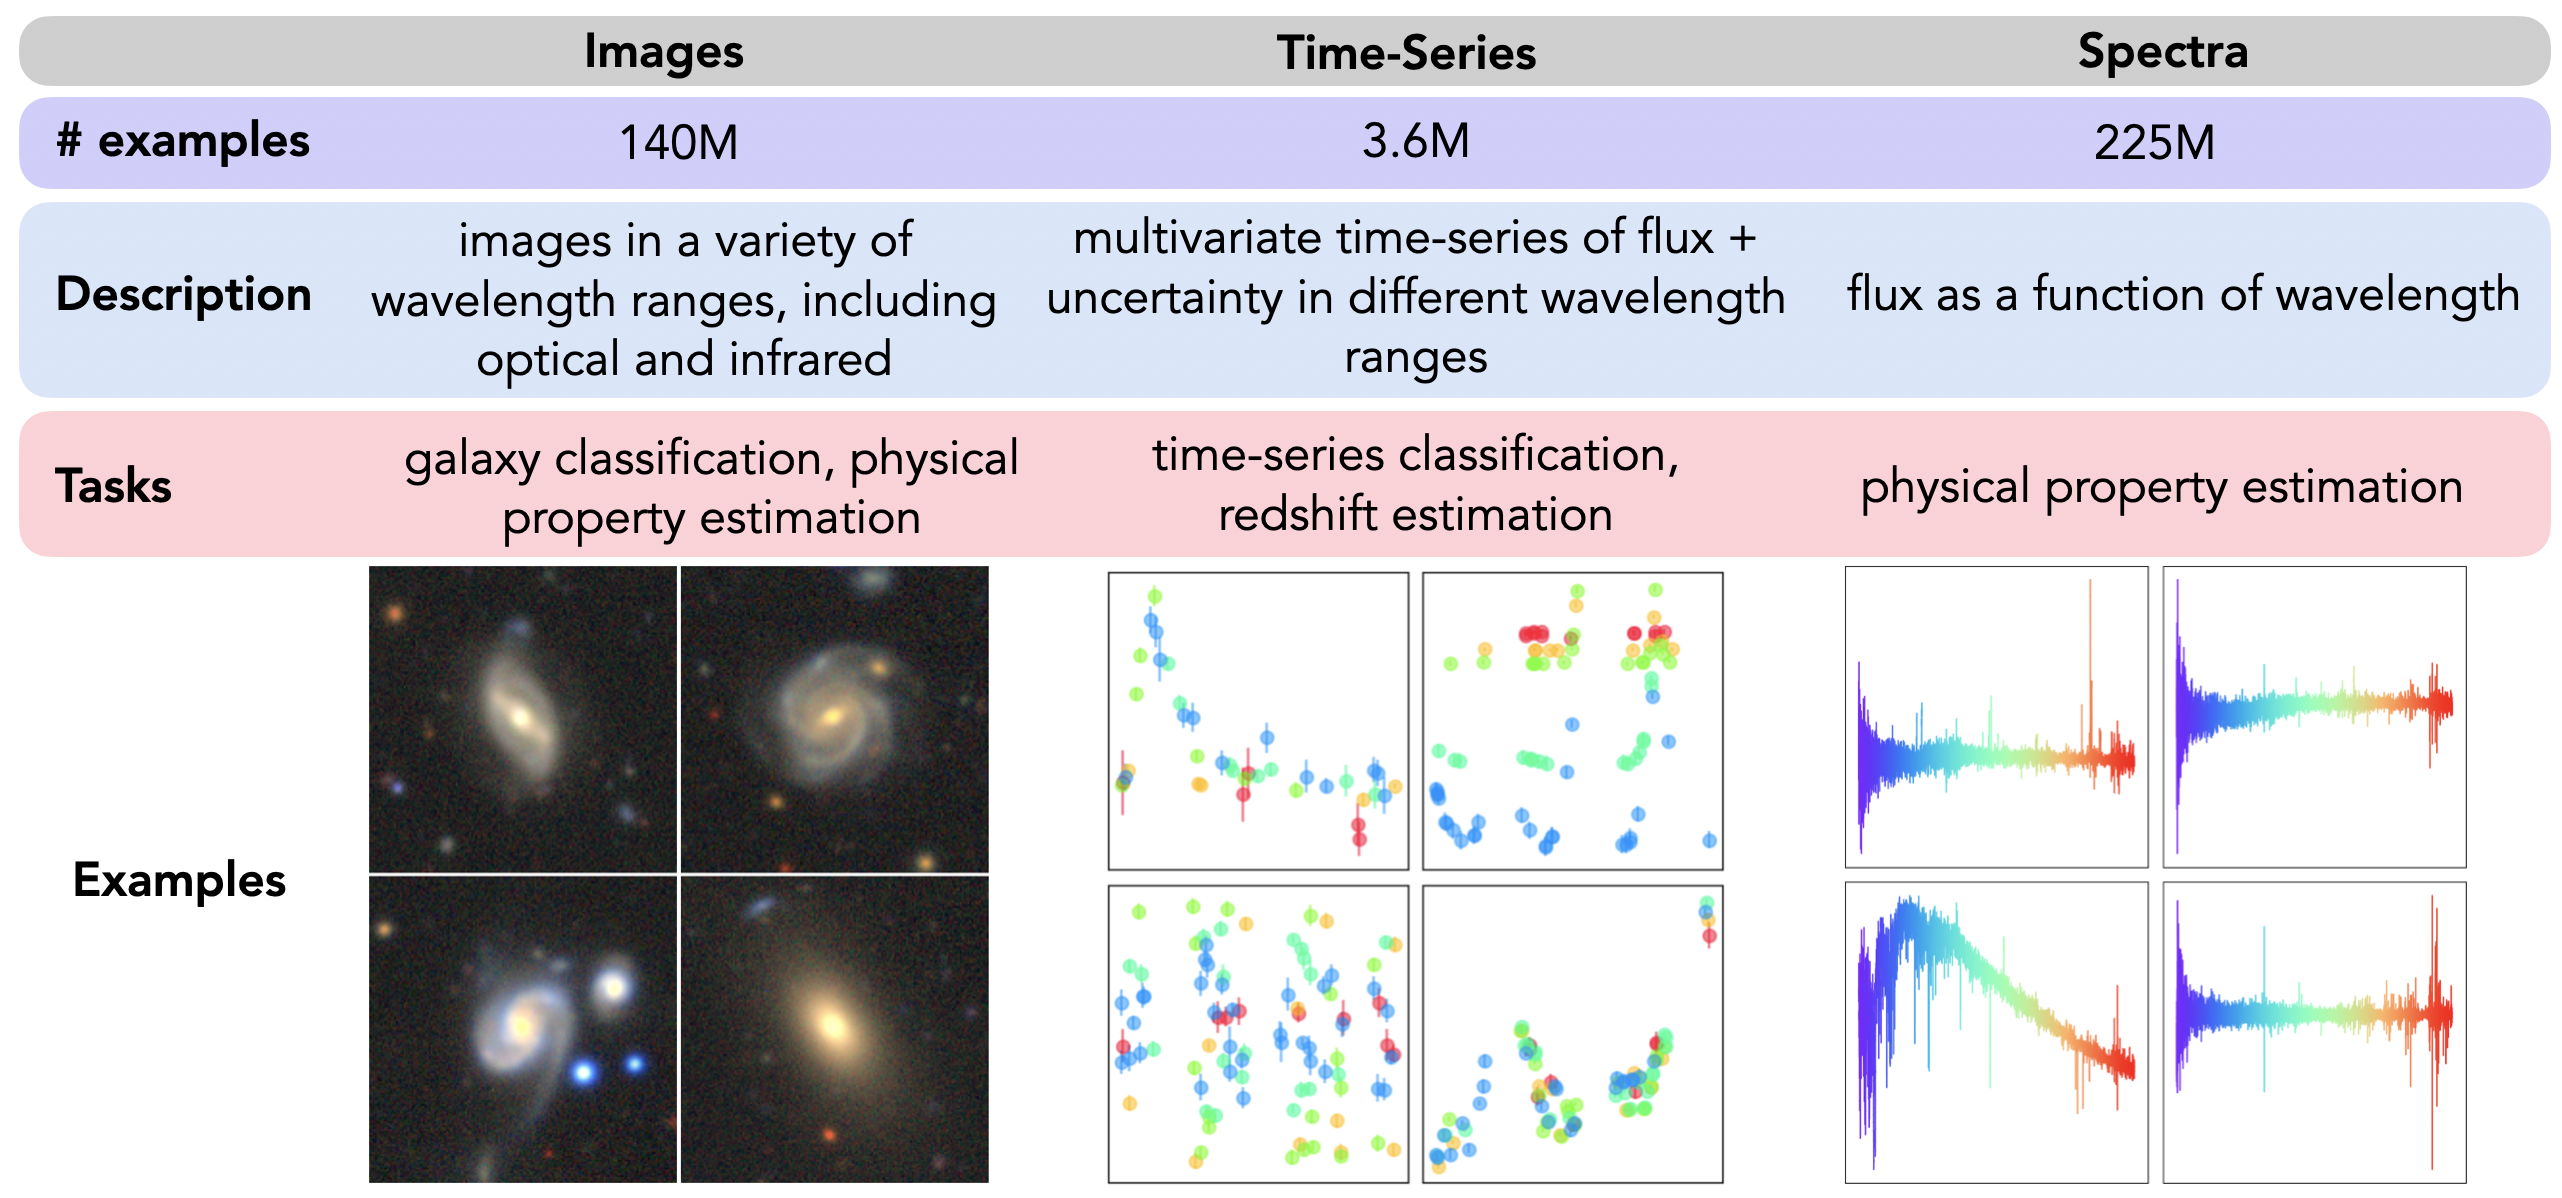
\includegraphics[scale=0.3]{paper/figures/dataset_examples.png}
    \caption{\small Illustration of the main modalities included in the \pile, along with typical associated machine learning tasks. In addition, the \pile also includes a small amount of hyperspectral images and tabular data, not shown here.}
    \label{fig:examples}
\end{figure}
% \begin{figure}
%     \centering
%     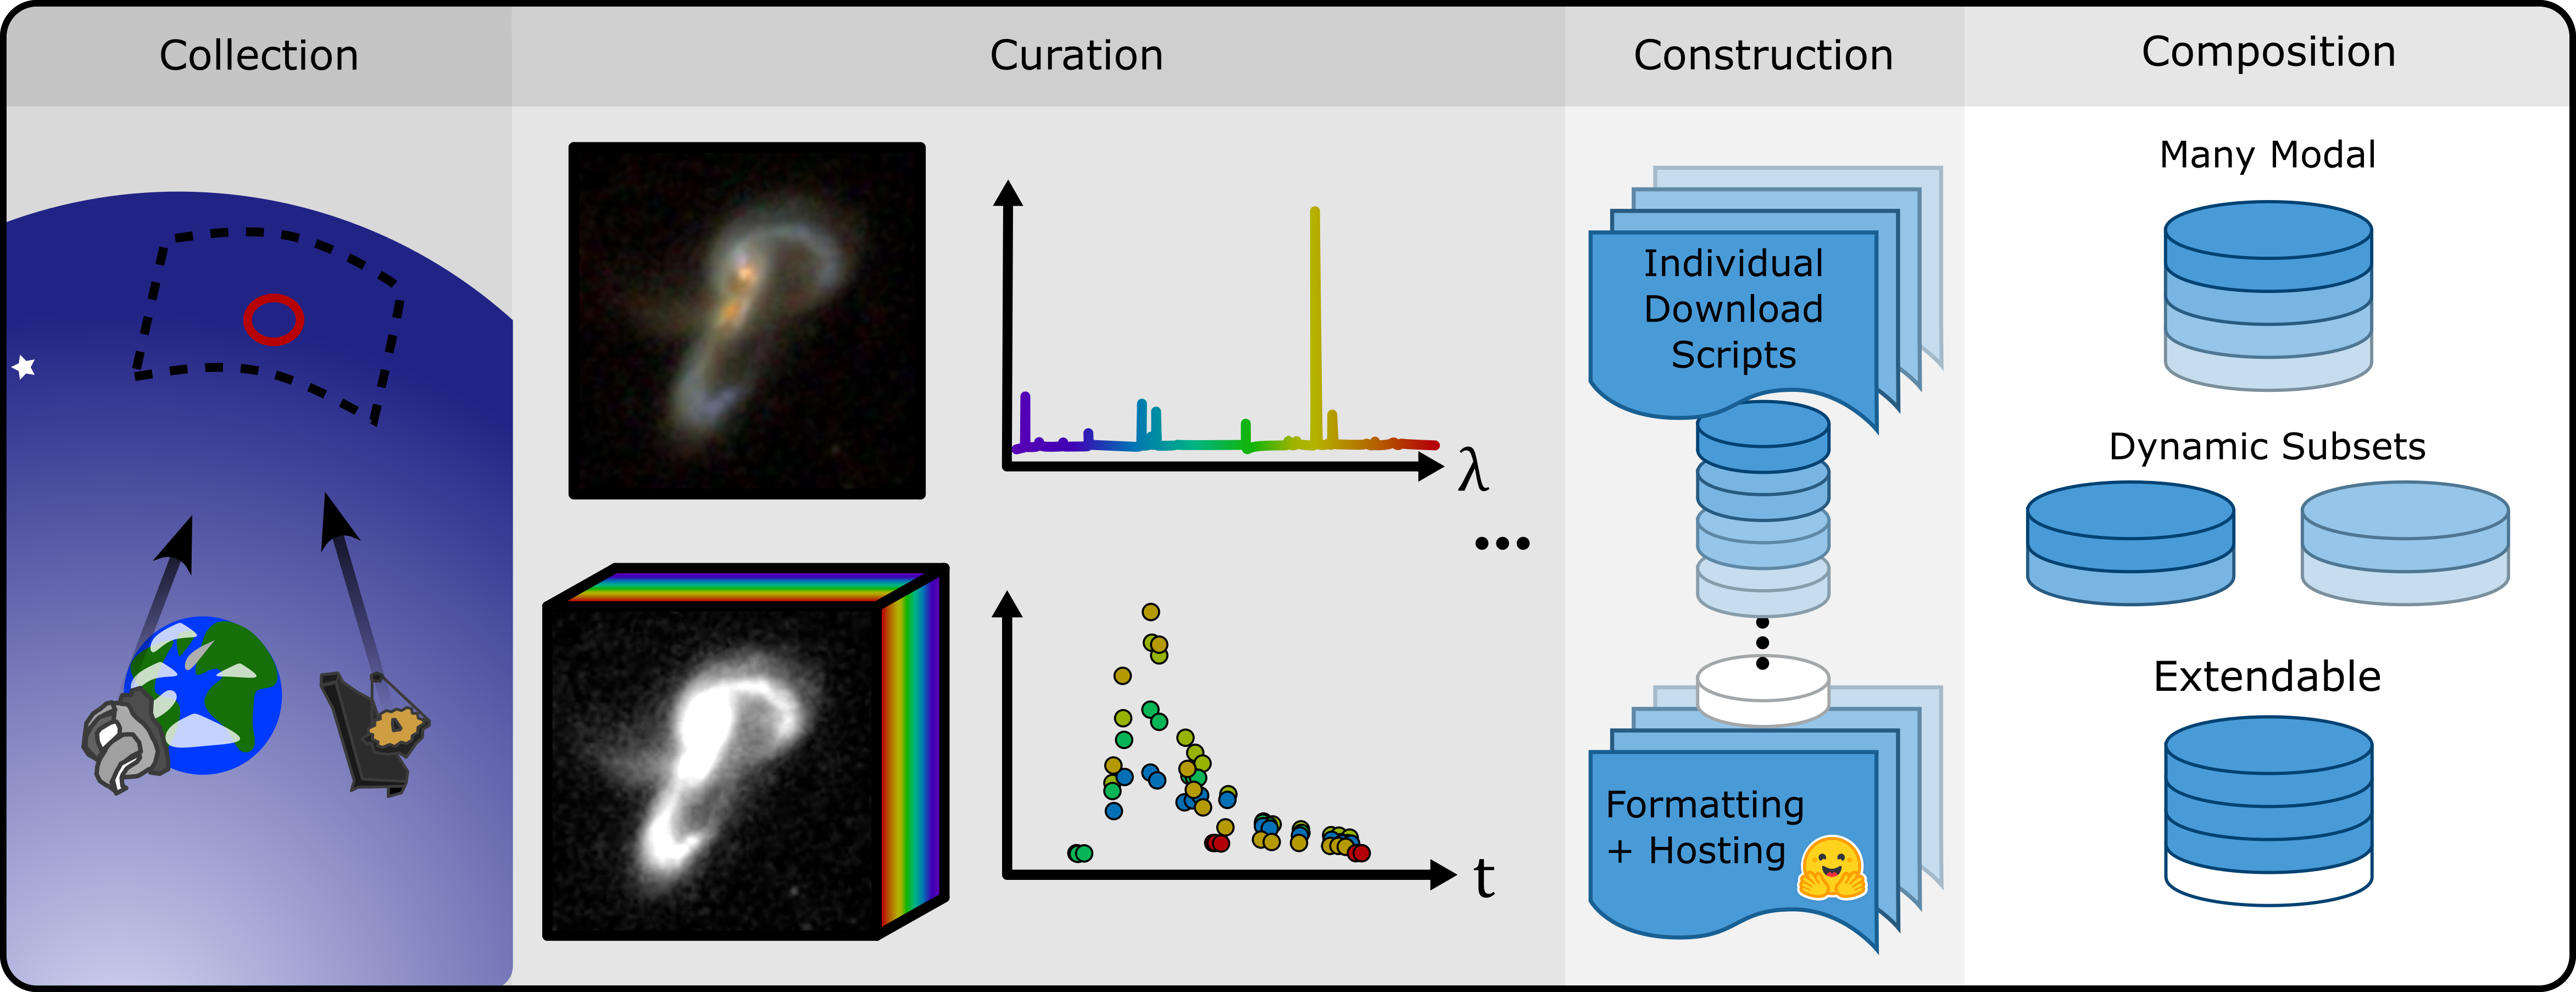
\includegraphics[width=1.0\linewidth]{paper/figures/opening_figure.png}
%     \caption{\small Illustration of \pile. Domain scientists with expertise in a given astronomical survey provide data download and formatting scripts available from \url{https://github.com/AstroPile/AstroPile}. All datasets are available as Hugging Face datasets sharing a common data schema for each modality and associated metadata. Users can generate any combination of \pile parent samples using provided cross-matching utilities.}
%     \label{fig:methodology}
% \end{figure}

In keeping with its scientific goals, the \pile also emphasizes the importance of relevant scientific ``metadata''. This includes relevant contextual information for each observation (e.g. observational noise, pixel scale, instrumental response, etc.) that not only helps preserve the dataset's utility for scientific ML but also enables the development of models that integrate information beyond the raw data level. In addition to the dataset, we also describe a range of benchmark tasks and baseline deep learning models that reflect current best practices in astrophysics. These benchmarks provide a foundation for evaluating new models, enabling researchers to compare their approaches against established standards and push the boundaries of what is possible with ML in astronomy.

Finally, extensibility and accessibility are core to the \pile project.
% puts significant emphasis on extendibility and ease of access of these datasets for the scientific community. 
All data subsets are accessible as standardized Hugging Face datasets. They can be downloaded locally in full or accessed as streaming datasets directly from the Hugging Face Hub, see \autoref{sec: availability and maintenance}. The code used to compile each component of the \pile from its respective official data source is hosted on the project's GitHub repository for transparency and reproducibility, and utilities to generate cross-matched (and multi-modal) versions of the dataset are also included. The architecture of the \pile source code is consistent, maintainable, and extensible.
This is in contrast to the common practice in the field, which is for independent researchers, groups, or collaborations to decide their data formats in isolation of one another, creating a significant barrier to entry for multimodal research in astronomy. By making \pile publicly available, we aim to catalyze innovation and collaboration among the astrophysics and ML communities. We believe that this dataset will not only advance our understanding of the universe but also contribute to the broader development of multimodal and metadata-aware ML methodologies.

\section{Related Work}

\paragraph{Scientific Machine Learning Datasets in Other Fields} Large curated and open datasets are gaining traction outside of the textual domain.
In remote sensing, Major-TOM \citep{francis2024} is a collated set of ESA Copernicus mission data that aims to standardise earth observation imagery into a common, ML-friendly format. Currently, Major-TOM comprises a combined 62\,TB of imagery. Like the \pile, Major-TOM is run as an open source project that the community can collectively contribute to.
In a similar vein, the MOMENT project \citep{goswami2024} introduces a large time-series dataset, as a publicly-available collection of 1.2B timestamps taken from 13 domains. These domains include---but are not limited to---medical information, economic indicators, power consumption, IoT weather data, speech, and general instrumental monitoring.

\paragraph{Large-Scale Machine Learning Datasets in Astrophysics} While astrophysics is inherently data-rich, most datasets have been compiled with traditional analyses in mind. This has resulted in data archives that are experiment-specific, non-uniformly stored, and not optimized for ML applications. Indeed, only a few exceptions exist where large datasets have been compiled for ML. For instance, \citep{Stein2021, Stein2022} introduced a substantial dataset of 76M images, enabling one of the first instances of self-supervised learning in astrophysics. Additionally, the PLAsTiCC \citep{PLAsTiCC_2018} light curve classification challenge is the largest collection of astronomical time-series data for ML research, with 3.5 million simulated light curves. Finally, the Galaxy Zoo project has provided large galaxy morphology classification datasets for ML \citep{gzchallengeKaggle2013, Walmsley2023GZDESI} that have been instrumental in various astronomy specific ML studies. This includes early astronomy applications of CNNs \citep{Dielman2015GZCNN}, Bayesian deep learning \citep{Walmsley2019BNN}, and modern neural scaling law analyses \citep{walmsley2024scaling,astropt}. However, none of these examples provide multimodal data, nor reach the scale of the data collected for the \pile.


\section{Creating a Large-Scale Dataset of Diverse Astronomical Data}

Modern astronomy has entered an era of large-scale, systematic surveys, supported by a range of space-based and ground-based instruments. These surveys generate unprecedented volumes of science-ready data products that are publicly available through open-access databases. However, these products are typically designed for conventional scientific workflows and not well-suited for ML applications; for example, astronomical imaging surveys typically provide full-frame mosaics from which individual uniform galaxy images must be cut out. As such, using these datasets effectively requires a high level of expertise and can be time-consuming. In addition, data structures and data access vary significantly among surveys, making it difficult to navigate diverse systems and interfaces to gather the necessary data. Therefore, to make use of astrophysical data, researchers must understand the intricacies of each separate survey and corresponding archive. This steep learning curve is a significant barrier to entry for ML applications in astrophysics, highlighting the need for a more streamlined and standardized approach to data access and preparation.

\subsection{Methodology}

\begin{figure}
    \centering
    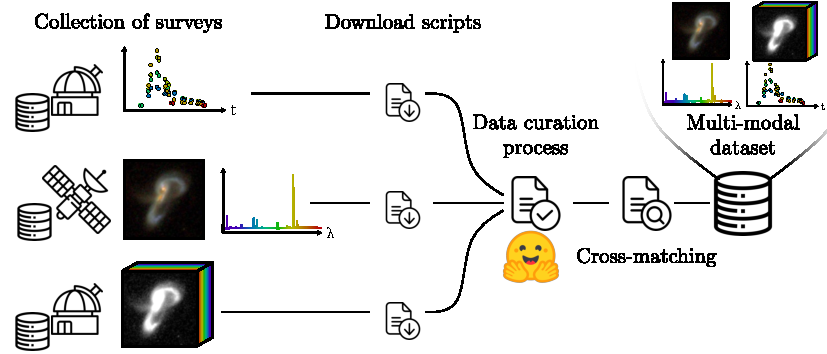
\includegraphics[width=0.98\textwidth]{paper/figures/astropile_data_processing.pdf}
    \caption{\small Illustration of the methodology behind the \pile. Domain scientists with expertise in a given astronomical survey provide data download and formatting scripts through Pull Requests on the project repository \url{https://github.com/MultimodalUniverse/MultimodalUniverse}. All datasets are then downloaded from their original source and made available as Hugging Face datasets sharing a common data schema for each modality and associated metadata. End-users can then generate any combination of \pile subsets using provided cross-matching utilities to generate multimodal datasets.}
    \label{fig:methodology}
\end{figure}

% Elements of context to convey:
%  - Most of astronomical data is stored in publicly available archives, however
% the raw data is not always reduced to a science-ready level. 
%  - Modern astronomy is structured around large surveys, which provide large
%  collections on homogeneous data
%  - But, in the way that data is stored and made available is not well suited to 
% machine learning applications. For instance, while it is common to have interfaces
% to query postage stamps, this is typically intended to be for visualisation, not 
% building datasets. 
%  - Furthermore, data is not always stored and presented in a similar fashion, interfaces to download data can vary greatly between surveys. 
%  - A great deal of expertise is required to know how to properly access each dataset
% and select scientifically relevant examples


\paragraph{Data Curation Strategy}
% Elements to convey here 
% - We are engaging a community of experts, who can all contribute their specific
% expertise in aggregating segments of the AstroPile
% - We are splitting the process into a fairly low barrier to entry for adding scripts that will download data from an official archive (that is, we are not too regarding on how code quality, such that this part does not require a software engineer) as long as it is reproducible, and clearly shows any selection/cuts of the original data going into the dataset
% - We make all data collection scripts publicly available, as it is often paramount in 
% scientific applications to understand exactly what selection effects might affect a sample
% - The next step after the data collection is to standardize the format of each data source to the lowest common denominator. In practice, this means that 1) we standardize all data to Hugging Face Datasets, 2) we further impose a data and metadata format that each modality must respect, as will be illustrated below. This allows us to standardize datatypes across different surveys and datasources, in a way that can then be ingested by a machine learning model
To overcome the barriers between different subfields and datasets imposed by the significant domain-specific scientific expertise required, we build the \pile by drawing on a community of diverse domain scientists. To facilitate their engagement, we have structured the data curation process to have a relatively low barrier to entry. Specifically, we enable domain scientists to contribute by simply adding scripts that download and process data from the official archives they know how to access into a standardized \pile format. While we do not impose stringent code quality requirements at this stage, it is essential that these scripts are reproducible and clearly document any selection or cuts applied to the original data. This approach allows researchers to contribute without extensive software engineering skills, as long as data collection is transparent and well-documented. All data collection scripts are publicly available to ensure the data curation process is reproducible. Once data is downloaded from its official repository, our data curation strategy involves adopting the HuggingFace Datasets framework and imposing a standardized format for each modality, ensuring compatibility across different surveys and ease of use for ML applications. 

\paragraph{Multimodal Cross-Matching}
% Elements to convey here
%  - Multimodailty is a crucial aspect of this dataset
%  - by and large, each survey is provided independent modality. 
%  - to make our dataset multi-modal, we cross-match observations based on their coordinates on the sky
%  - Contrary to what is possible for large text-image datasets, the intersection of different datasets is limited. For instance, we only have ~4M spectra in total, so we can't associate a spectrum to all images. We can't provide a large scale datasets joining all 
%  - We provide a set of utilities that will allow for this cross-matching in an efficient manner. 
%  - Because there are many ways to build cross-modal datasets, and that the more modalities we add, the fewer the samples, it is important to leave to the end-user the ability to extract cross-matched datasets for their specific applications.
Multimodality is a crucial aspect of the \pile, but it presents several challenges. Specifically, each astronomical survey provides data in a single modality; therefore, to build multimodal examples, it is necessary to cross-match observations from several sources. Fortunately, a fundamental property of every survey is the provision of sky coordinates for each observation, enabling cross-survey matching via coordinate matching. However, the intersection between two or more surveys is often relatively small. This limitation inherently prevents the collection of dataset pairs on the scale of projects like Laion-5B \cite{Schuhmann2022}, primarily because some modalities are much more expensive to acquire than others. Consequently, it is essential to provide access to large-scale unpaired datasets, along with the tools to easily generate various multimodal dataset pairings. The \pile addresses this need by offering a set of common cross-matched datasets and utilities that enable end-users to generate custom cross-matches tailored to their specific scientific applications. This approach ensures flexibility and maximizes the dataset's utility across different research needs.

\autoref{fig:methodology} summarizes the steps of our data curation and data access methodology.

\subsection{Overview of the Dataset}

\autoref{tab:data_summary} provides a breakdown of the different scientific modalities included in the \pile, along with a description of their origin and their scientific relevance. Overall, the \pile represents 70 TB of data, largely dominated by 60TB of multi-band imaging.

% \begin{figure}
%     \centering
%     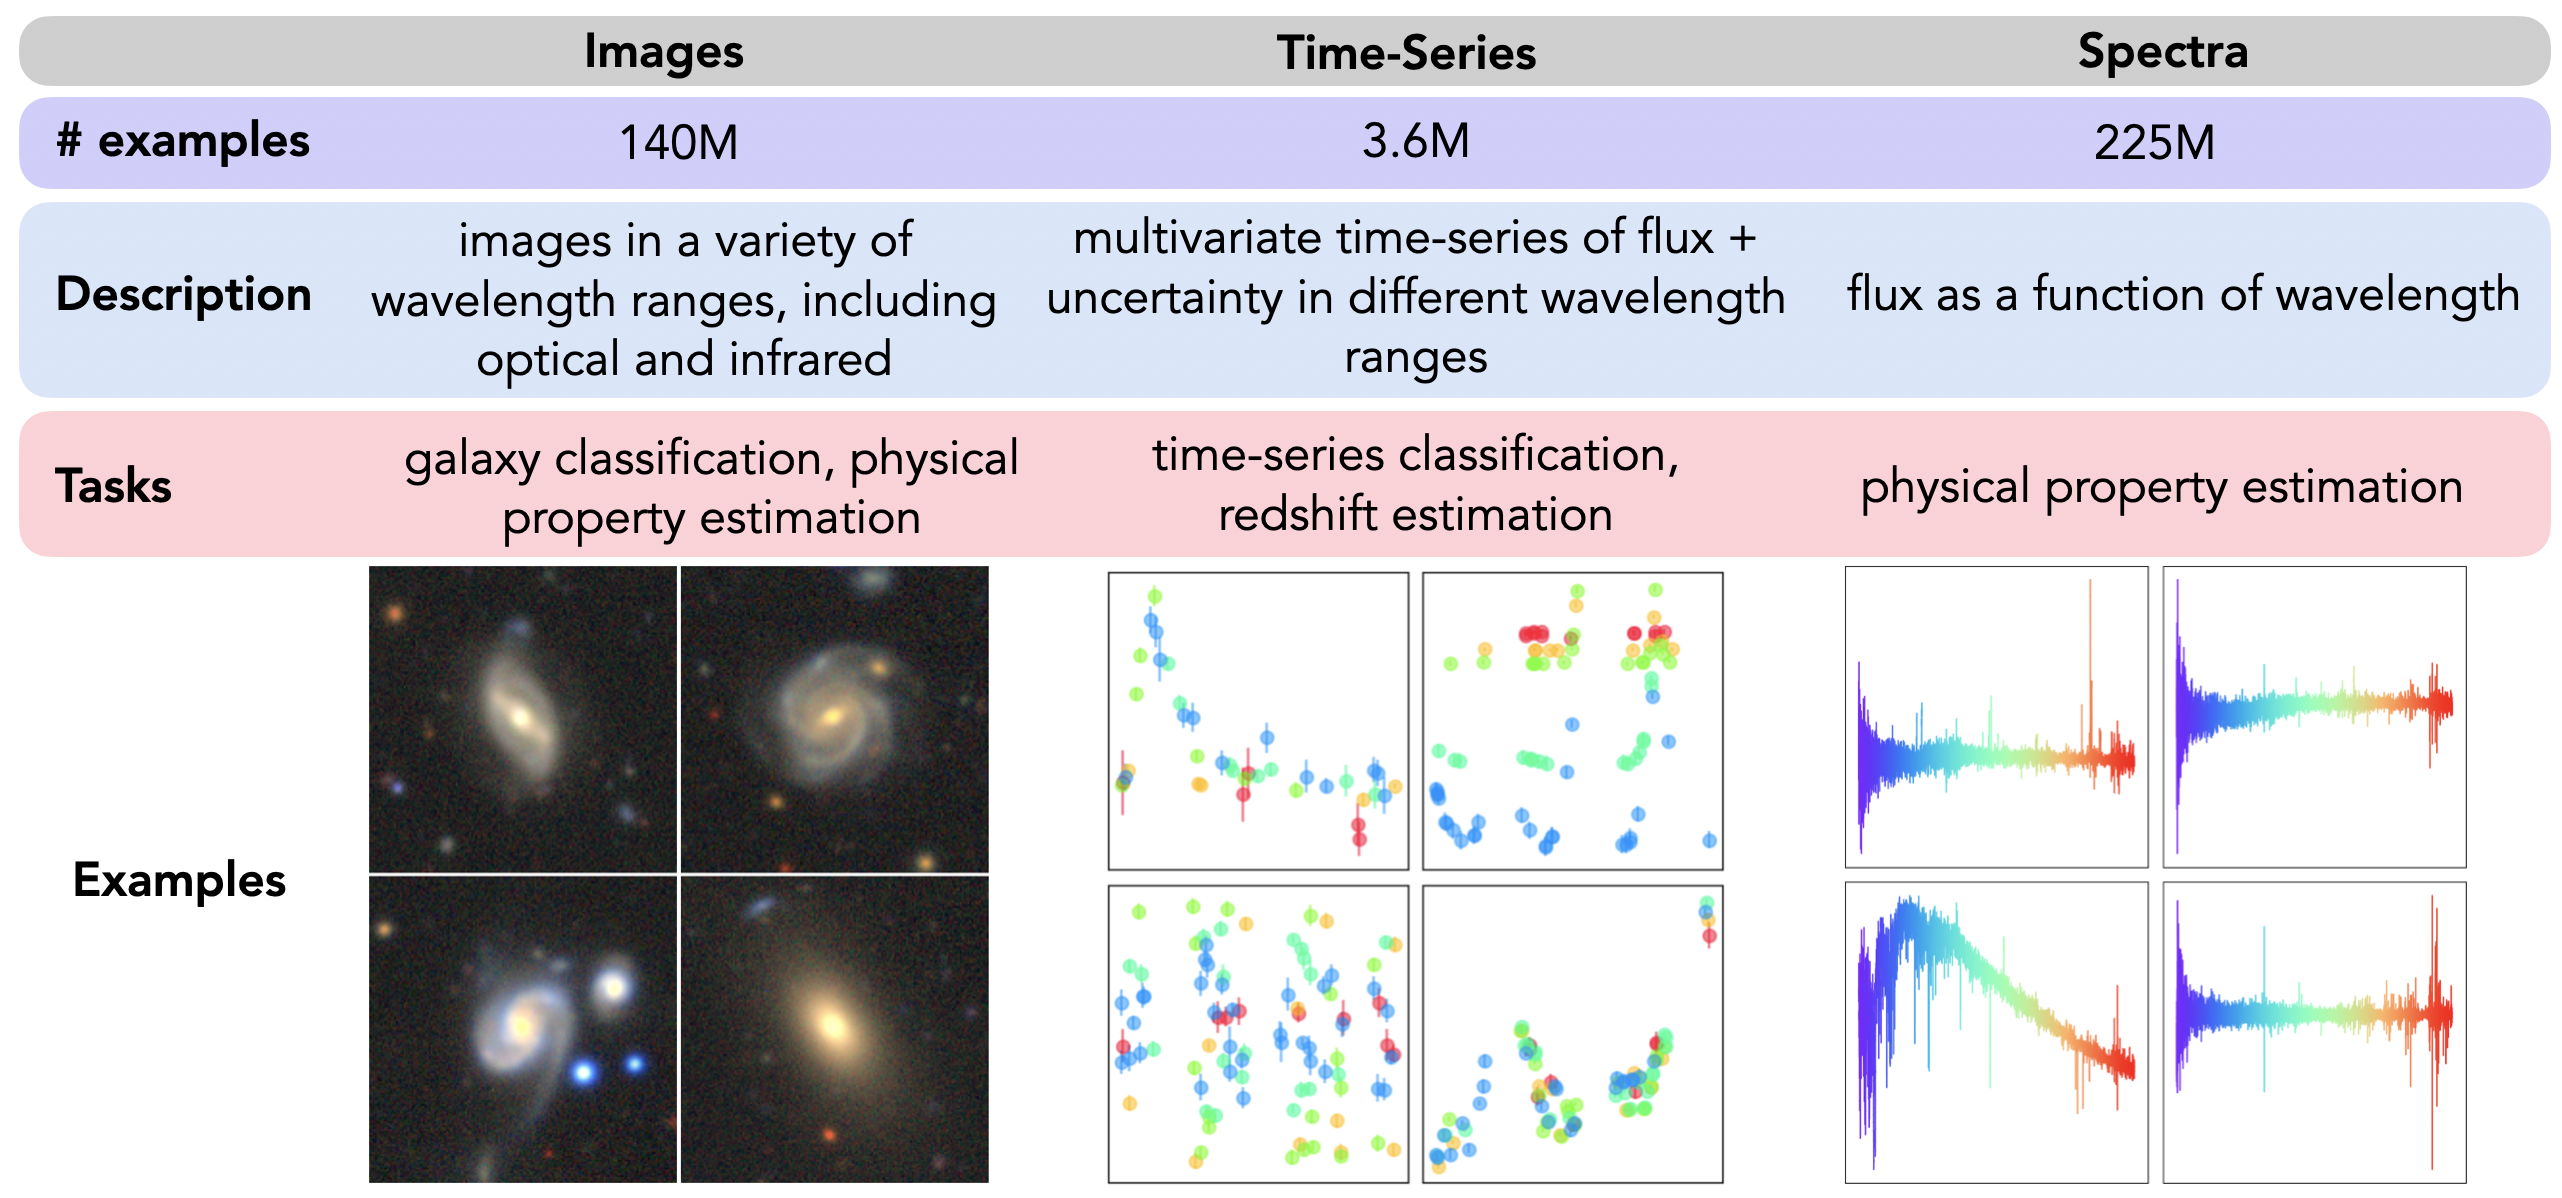
\includegraphics[scale=0.3]{paper/figures/dataset_examples.png}
%     \caption{Overview of the modalities included in the Multimodal Universe. We present examples of ML tasks for each modality and set up benchmarks to evaluate models for each of these tasks. The Multimodal Universe also includes a small amount of hyperspectral image data and tabular data, which are not shown here.}
%     \label{fig:examples}
% \end{figure}

\begin{table}[ht]
    \begin{threeparttable}[b]
    \centering
    \rowcolors{2}{verylightgray}{white}
    \resizebox{\textwidth}{!}{
    \begin{tabular}{c l c c c c}
        \toprule
          &  &  & & Number of & Main  \\
        \multirow{-2}{*}{Modality} & \multirow{-2}{*}{Source Survey} & \multirow{-2}{*}{N_c} & \multirow{-2}{*}{Shape} & samples  & science 
         \\\midrule
         \cellcolor{white} & Legacy Surveys DR10 \citep{DESILS} & 4 & 160\texttimes160 & 124M & Galaxies \\
         \cellcolor{white} & Legacy Surveys North \citep{DESILS, Stein2021} & 3 & 152\texttimes152 & 15M & Galaxies \\
         \cellcolor{white}{\small Images } & HSC~\citep{2018PASJ...70S...4A, HSCPDR3} & 5 & 160\texttimes160 & 477K & Galaxies \\
        \cellcolor{white} & BTS~\citep{Fremling20, Perley20, BTSbot_2024} & 3 & 63\texttimes63 & 400K & Supernovae \\
         \cellcolor{white} & JWST\citep{2023ApJ...946L..12B,2024ApJ...965L...6B,2023arXiv230602465E} &  6-7 & 96\texttimes96 & 300K & Galaxies \\
         \arrayrulecolor{black!30}\midrule
        \cellcolor{white} & Gaia BP/RP~\citep{2023AA...674A...1G} & - & 110\tnote{1} & 220M & Stars \\
         \cellcolor{white} & SDSS-II~\citep{2009ApJS..182..543A} & - & Variable & 4M & Galaxies, Stars \\
        \cellcolor{white} {\small Spectra} & DESI~\citep{2016arXiv161100036D} & - &  7081 & 1M & Galaxies \\
        \cellcolor{white} & APOGEE SDSS-III~\citep{2015ApJS..219...12A} & - & 7514 & 716k & Stars \\
        \cellcolor{white} & GALAH \citep{GALAH_Buder} & - & Variable & 325k & Stars \\
        \cellcolor{white} & Chandra \citep{CSC} & - &  Variable & 129K & Galaxies, Stars \\
        \cellcolor{white} & VIPERS~\citep{scodeggio2018vimos} & - & 557 & 91K & Galaxies \\

        \arrayrulecolor{black!30}\midrule
        \cellcolor{white}\multirow{-1}{*}{{\small Hyperspectral Image }} & MaNGA SDSS-IV~\citep{2022ApJS..259...35A} & 4563 & 96\texttimes96 & 12k & Galaxies \\
        \arrayrulecolor{black!30}\midrule
        \cellcolor{white} & PLAsTiCC\tnote{2} \citep{PLAsTiCC_2018}& 6 & Variable & 3.5M & Time-varying objects \\
        \cellcolor{white} & TESS \citep{ricker2015, Caldwell2020} & 1 & Variable & 160K & Exoplanets \\ 
        \cellcolor{white} & CfA Sample \citep{CfA3, CfA4, CfA-SECCSN, CfA-SNeII} & 5-11 & Variable & 1K & Supernovae \\
        \cellcolor{white} & YSE \citep{YSE_DR1_2023} & 6 &  Variable & 2K & Supernovae \\
        \cellcolor{white} & PS1 SNe Ia \citep{PS1} & 4&  Variable & 369 & Supernovae \\
        \cellcolor{white} {\small Time Series} & DES Y3 SNe Ia \cite{DESY3SN} & 4 &  Variable & 248 & Supernovae \\
        \cellcolor{white} & SNLS \citep{SNLS} & 4 & Variable & 239 & Supernovae \\ 
        \cellcolor{white} & Foundation \citep{foundation2018,foundation2019} & 4 & Variable & 180 & Supernovae \\
        \cellcolor{white} & CSP SNe Ia \citep{CSP-I_2010, CSP-I_2011, CSP-I_2017} & 9 & Variable & 134 & Supernovae \\
        \cellcolor{white} & Swift SNe Ia\citep{Sousa}& 6 & Variable & 117 & Supernovae \\
        % \cellcolor{white} & CfA 4 SNe Ia  & Variable & 341 & Supernovae \\
        % \cellcolor{white} & CfA 3 SNe Ia  & Variable & 185 & Supernovae \\
        % \cellcolor{white} & CfA Stripped-Core SNe & Variable & 249 & Supernovae \\
        % \cellcolor{white} & CfA SNe II & Variable & 400 & Supernovae \\       
        \arrayrulecolor{black!30}\midrule
        \cellcolor{white} & Gaia~\citep{2023AA...674A...1G} & - & - & 220M & Stars \\
        \cellcolor{white} {\small Tabular} & PROVABGS~\cite{Hahn_2023}& - & - & 221K & Galaxy \\
        \cellcolor{white} & Galaxy10 DECaLS~\cite{2022MNRAS.509.3966W, leung_galaxy10_decals} & -  & - & 15K & Galaxy \\
        \bottomrule
    \end{tabular}}
    \caption{\small Summary of samples included in the \pile, details of all samples are provided in appendix. 
    % {\small 
    N$_c$ indicates the number of channels of a given observation.  [1] These are represented as 110 basis coefficients that can be resampled to an arbitrary wavelength grid. [2] Simulated dataset.
    % [3] See Appendix~\ref{app: time-series data} for a full breakdown of the CfA Sample.
    }
    % }
    \label{tab:data_summary}
    \end{threeparttable}
\end{table}

We provide below further description of these modalities and summarize the standardized fields and metadata defined for the main modalities of the \pile in \autoref{tab:fields_metadata}. A complete description of the schema for each modality in the dataset is further provided in appendix.

% FL: I'll condense in one table the content of the different key fields for the main modalities, it will save space compared to different listings, if it's still too detailed, we can move it to the appendix.


% \subsubsection{Optical and Infrared Imaging}

\paragraph{Optical and Infrared Imaging} Astronomical images are obtained via cameras installed at the focal plane of both space and ground-based telescopes, that capture photon emission from distant astronomical sources. An observed image $I$ can be described as: $I = S \ast \Pi + n $ where $S$ is the intrinsic source emission on the sky, $n$ is the measurement noise, and $\Pi$ is the instrumental response of the telescope, also known as the Point Spread Function (PSF). The PSF is at minimum characterized by its full width half maximum (fwhm), which sets the spatial resolution of the image. In addition, these images are typically acquired in a number of specific broad wavelength ranges, referred to as bands or channels. Knowledge of the bands, PSF, noise properties, and pixel scale, are generally required to fully characterize an observation and take into account the specificities of a particular instrument or observatory. Compared to natural images, astronomical images are typically noisier, and exhibit a large dynamic range, generally spanning several orders of magnitude between the bright objects and fainter sources.

% \paragraph{Description} Imaging is the most common data type in astronomy. Astronomical images are obtained with CCD cameras installed in the focal planes of telescopes both in space and in the ground which capture the photons emitted by distant astronomical sources. The formation of an image is often described as: 

% \begin{equation}
% I(x, y) = \left( S(x, y) \ast PSF(x, y) \right) + N(x, y)
% \end{equation}

% where: \( I(x, y) \) is the intensity of the image at position \((x, y)\) in the focal plane, \( S(x, y) \) is the intrinsic source emission at position \((x, y)\), \( PSF(x, y) \) is the point spread function of the telescope, \( N(x, y) \) is the noise at position \((x, y)\) and \(\ast\) denotes the convolution operation. \\
% A telescope is therefore fully characterized by its impulse response or PSF which in the case of ground based facilities includes the effect of the atmosphere and the telescope optics, while in space it only measures the optical structure. The PSF is at minimum characterized by its full width half maximum (fwhm) which typically sets the spatial resolution of the image. In addition, astronomical images are usually taken with filters that allow only photons of a specific wavelength (or energy) to go through. This is because every wavelength carries a different physical information. An astronomical imaging survey is therefore composed of different images of the same sources observed in different filters. The most common surveys cover the optical and near-infrared part of the spectrum but there exist also X-ray or radio surveys. \\
% Compared to natural images, astronomical images have some specific properties which usually require specific treatments for ML applications. First, the dynamic range of the pixel values generally spans several orders of magnitude between the central parts of a source and the outskirts. Second, in most of the cases, the signal to noise ratio is very low and can therefore vary drastically depending on the brightness of the source of interest, even on a given dataset. \\

% In \pile, the imaging dataset, in addition to the image itself (array) has a common structure with the following information about the filter used (band), the fwhm of the PSF (fwhm) and the size of the pixels in arcsec, as summarized in \autoref{tab:fields_metadata}.
% % \begin{lstlisting}[language=Python, caption=Dictionary Structure for all Imaging Datasets, basicstyle=\ttfamily\footnotesize, keywordstyle=\color{blue}, commentstyle=\color{green!50!black}, stringstyle=\color{red}]
% % features = {
% %     "image": Sequence(
% %         feature={
% %             "band": Value("string"),
% %             "array": Array2D(
% %                 shape=(self.config.image_size, self.config.image_size), 
% %                 dtype="float32"
% %             ),
% %             "psf_fwhm": Value("float32"),
% %             "scale": Value("float32"),
% %         }
% %     )
% % }
% % \end{lstlisting}
% When additional useful information is provided along with the main modality in a specific survey, that information is included as optional, non-standardized fields. The user is then directed to the original source of the data for a specific description of these fields and their meaning. 

% \paragraph{Sources} We collect a diverse set of imaging sources, spanning ground- and space-based observatories, across multiple wavelengths. Specifically from ground-based surveys, we primarily rely on the Legacy Survey\FL{cite}, which provides extensive imaging data of the northern and southern skies, the Hyper Suprime-Cam (HSC) SSP survey \FL{cite} which provide higher resolution and less noisy images but on a smaller fraction of the sky, and data from the Bright Transient Survey Bot (BTSbot) \FL{cite} which provides a link between imaging and time series data. In addition, we include space-based imaging from the James Webb Space Telescope, which provides an exquisite but fairly smaller sample of high-resolution infrared images.

% \paragraph{Examples of Scientific use-cases} 
% Images are used for a variety of scientific applications in all fields of astrophysics. For example, accurately measuring the shapes of galaxies on large samples provides information about the geometry of the universe. By looking at the detailed structure of galaxies, we can put constraints on their assembly histories. The total number of photons emitted in different filters inform about the distance and the physical properties of the source. 

% \subsubsection{Spectroscopic data} 

\paragraph{Spectroscopy} Similarly to imaging data, light from distant objects is gathered and focused first by the telescope, but instead of being directly imaged with a camera, the light from cosmic objects is dispersed into various wavelengths or energies using a spectrograph. A spectrum is therefore a 1-d signal representing the decomposition of the light from an object as function of wavelength or energy of the photons. Similarly to images, a measured spectrum $y$ is the result of the following observational process: $y = L \ast x + n$ where $L$ is the instrument's impulse response (also known as Line Spread Function; LSF) and $n$ is a measurement noise. Contrary to images, where the absolute position of each pixel on the sky is not directly needed to interpret the signal, for spectroscopy knowledge of absolute  wavelength corresponding to each pixel is crucial, which is why each spectrum not only provides a array of measured flux $y$ but also the corresponding wavelength array $\lambda$. 
%For photon-counting detectors, as in the case of X-ray telescopes, spectra are more typically expressed as function of energy than wavelength, but. % can be obtained by directly computing the distribution of individual photon energies and convolving with the telescope's sensitivity over the energy range.  %  The spectrum of an object is a histogram of the number of photons per wavelength or energy bin. 
% Therefore, at first glance, the spectrum of a distant object would look like a 1-D time series, but its x-axis is not time, but wavelengths or energy, while y-axis is flux, the amount of electromagnetic radiation, in that wavelength bin. 

% \paragraph{Sources} We include a range of spectroscopic measurements in the dataset, starting with ground-based surveys in the optical and near infrared Sloan Digital Sky Survey, APOGEE and the Dark Energy Spectroscopic Instrument \FL{cite}. In addition, we also include X-ray spectra from the Chandra space-based observatory, and a large number of measurements from the Gaia space-based observatory \FL{cite,cite}. 

% \paragraph{Examples of Scientific use-cases} Complementary to images, spectroscopic observations provide a wealth of information on the composition and physical properties of astronomical objects. It is in particular possible to measure from spectra how much the light from distant galaxies has been shifted towards the red by the cosmic expansion of the Universe, which tells us about their distance with respect to the observer. The spectrum of galaxies also encodes information about their stellar populations, and in turn about their formation and evolution history. In a different regime, X-ray spectra of the light emitted by the accreting gas around compact object such as black holes or neutron stars convey valuable information about such systems. 

% emission is produced near compact objects that are accreting gas from their surroundings, such as black holes or neutron stars. The radiation is either thermal emission from a very hot accretion disk, or non-thermal emission resulting from the acceleration of charged particles as they are accreted into the compact object. The distribution of the X-ray photon energies (i.e., the X-ray spectrum) can inform about the amount of accretion taking place, the temperature of the disk, or even the rotation of the compact object.
% A few interesting points to note for the general scientific community is that usually, a spectrum of a planet, a star, or a galaxy contains a wealth of information about that object: 
% \begin{itemize}
% \item Redshift: this describes how far away the object is from earth. As an astronomical emits light, the further the object is from us, its light will be further stretched, turning it into lower frequency, thus making it redder, and shifting to the redder side of the spectrum, more well-known as Doppler effect. At cosmological scales, as the distant objects recess away from us, the cosmological redshift is then interpreted as the Doppler shift with this recession. 

% \item Star-forming history and properties of the galaxies: 
% The galaxy spectrum can be broadly thought of as a combination of the continuum of the galaxy and the emission and absorption lines. These emission and absorption line features are used to derive the history and properties of the galaxy, such as how star-forming was happening and when; what kind of surrounding medium are at the galaxy will also determine the absorption lines that will be observed. These lines are representative of the chemical reactions that are taking place in or around the galaxy at certain temperatures and environment while being indicative of the existence of certain materials. 

% \item Properties of accreting black holes:
% X-ray emission is produced near compact objects that are accreting gas from their surroundings, such as black holes or neutron stars. The radiation is either thermal emission from a very hot accretion disk, or non-thermal emission resulting from the acceleration of charged particles as they are accreted into the compact object. The distribution of the X-ray photon energies (i.e., the X-ray spectrum) can inform about the amount of accretion taking place, the temperature of the disk, or even the rotation of the compact object.
% \end{itemize}


% \subsubsection{Hyperspectral imaging} 

\paragraph{Hyperspectral imaging} Hyperspectral imaging is a data modality that combines imaging and spectroscopy to produce spatially resolved spectra in a two-dimensional region. It uses an Integral Field Unit (IFU) to produce a three-dimensional "datacube" consisting of 2d array of spatial pixel elements, i.e "spaxels", each containing a spectrum in a specific wavelength range. IFUs provide a wealth of information. For example, by analyzing the spectrum within each spaxel, one can produce "images" of spectral features and derived parameters, such as emission/absorption lines and the velocities of gas and stars in the galaxy. By aggregating spectra together within specific spatial regions, one can compare the properties (such as star forming rates) of different physical regions of the galaxy. By extension of both images and spectra, hyperspectral images are accompanied by an instrumental response in the form of both Point Spread Function and Line Spread Function information.

\paragraph{Time-Series}
Time series data, often called light curves (brightness over time), are commonly examined when astronomical objects or events vary in brightness in time. These include relatively short-lived, explosive transients such as supernovae (exploding stars) and tidal disruption events, long-lived sources that show stochastic variation over time such as active galactic nuclei and quasars, and (quasi-)periodic sources such as pulsating stars and exoplanets. These time series are a sequence of flux (i.e. intensity) measurements. Because of their unique properties, astronomical time-series pose a challenge to traditional ML architectures. For one, most light curves are sparsely and irregularly sampled in both time and wavelength due to the unique survey strategy of each telescope. Flux measurements are also often plagued with large uncertainties, especially those from faint sources. Finally, data from different telescopes are highly heterogeneous and thus difficult to combine (e.g., to build a larger training set for ML applications). Together, these factors make our time-series data products a compelling and challenging dataset for ML researchers.

% However, some time series comprise spectroscopic measurements, although these are a small minority due to the increased observational expense. %, which are analysed to calculate the total apparent brightness of an astronomical source in a given image. By observing the same source repeatedly over time, it is possible to construct a time series showing how the luminosity of a source evolves over time. These can be 

% \paragraph{Sources.}
% The Multimodal Universe includes type Ia supernovae samples from:
% \begin{itemize}
%     \item Pan-STARRS (PS1):
%     \item Dark Energy Survey (DES):

%     \item Swift
%     \item CSP
% \end{itemize}
% We also include datasets of multiple supernova types from:
% \begin{itemize}
%     \item Young Supernova Experiment (YSE)
%     \item SuperNova Legacy Survey (SNLS):
%     \item Foundation
%     \item Center for Astrophysics Supernova sample
    
% \end{itemize}
% In addition, we include a simulated dataset of a broader variety of astronomical time-varying phenomena from the Photometric LSST Astronomical Time-series Classification Challenge (PLAsTiCC).

% \paragraph{Scientific Use-Cases}


% In addition to inter-survey differences, targets within the same survey are observed heterogeneously due to factors like weather, seasonal availability, and telescope scheduling.
% This leads to a significant disparity between the most densely and sparsely covered light curves.

% Lastly, astronomical time series 
% differ from time series in many other fields in that the relationship between time stamps and photometric measurements is often one-to-one instead of one-to-many.
% As an example of the latter relationship, multiple stock prices can be indexed to a single time.
% It is possible to conduct simultaneous observations in multiple filters or with multiple telescopes, but the typical procedure is to perform multiple observations serially, which produces unique time stamps for each measurement of each object.

% shown in Listing~\ref{lst:time-series}.
% \begin{lstlisting}[label={lst:time-series},language=Python, caption=Dictionary Structure for all Time Series Datasets, basicstyle=\ttfamily\footnotesize, keywordstyle=\color{blue}, commentstyle=\color{green!50!black}, stringstyle=\color{red}]

% features = {
%     'lightcurve': Sequence(
%         feature={
%             'band': Value("string"),
%             'flux': Value("float32"),
%             'flux_err': Value("float32"),
%             'time': Value("float32")
%         }
%     ),
%     'object_id': Value("string"),
%     'obj_type': Value("string"),
% }
% \end{lstlisting}
%    'ra': Value("float32"),
%    'dec': Value("float32"),
% The ``flux'' feature describes the brightness of a target on a linear scale, but sometimes this and the ``flux\_err'' feature are replaced with ``mag'' and ``mag\_err'' features which measure brightness on a logarithmic scale given by
% \begin{equation}
% \begin{split}
%     \textrm{mag} & = \textrm{ZP} - 2.5\log_{10}(\textrm{flux}) \\
%     \textrm{mag\_err} & = 2.5\log_{10}(1+\textrm{flux\_err} / \textrm{flux})
% \end{split}
% \end{equation}
% where ZP is an arbitrary zero point defined where flux is 1.
% Unless explicitly stated otherwise, the ZP used across all datasets is 27.5.
% As with the Optical/NIR Images, some time series datasets within the \pile have additional metadata such as redshift.
% Also emphasizing all the difficulties of astronomical data (dynamic range, high noise)
% 

% \paragraph{Tabular data} \FL{add short description}
\paragraph{Tabular data} The \pile also aggregates large catalogs of tabular data from different sources, corresponding either to particular measurements (e.g. measured flux for a particular object), or the result of the processing of these observations by an analysis pipeline (e.g. calculations of galaxy properties or reporting of galaxy morphology)\footnote{We do not enforce standard definitions for tabular data
% as these measurements are not uniform across surveys, 
and instead refer the user to the original survey description.}. 



\begin{table}[]
    \begin{threeparttable}[b]
    \centering
    \rowcolors{2}{verylightgray}{white}
    \begin{tabular}{c c l}
        \toprule
        Modality & Field & Description
        \\
        \midrule
         \cellcolor{white} & flux & Array of flux measurements of the image \\
         \cellcolor{white} & ivar & Inverse variance of noise in the image \\
        \cellcolor{white} Images & band & Key indicating the wavelength range of the image \\
         \cellcolor{white} & psf\_fwhm & Size of the instrumental response (Point Spread Function) \\
         \cellcolor{white} & scale & Scale of pixels on the sky
         \\\arrayrulecolor{black!30}\midrule
        \cellcolor{white} & flux & Measured flux as a function of wavelength \\
        \cellcolor{white} Spectra & ivar & Inverse variance of noise on measured flux \\ 
        \cellcolor{white} & lsf\_sigma & Size of the instrumental response (Line Spread Function) \\
        \cellcolor{white} & lambda & Wavelength of each flux measurement \\\arrayrulecolor{black!30}\midrule
        \cellcolor{white} & flux  & Measurements of flux as a function of time \\ 
        \cellcolor{white} Time  & flux\_err & Uncertainty on flux measurement \\
        \cellcolor{white} Series & band & Key indicating the wavelength range of the measurement \\
        \cellcolor{white} & time & Time of observation \\
         \bottomrule
    \end{tabular}
    \caption{\small Description of standardized fields and metadata provided for the main modalities. These fields represent necessary and near-sufficient information to allow for the consistent interpretation of observations from multiple surveys or instruments.}
    \label{tab:fields_metadata}
    \end{threeparttable}
\end{table}

% \FL{TODO: include breakdown of the data, mention the distinction between large scale datasets, and smaller surveys which may be used for fine-tuning.}
% Points to communicate here:
% - Overall data breakdown
% - Some datasets are functionally there for foundation model training
% - Others are going to support fine tuning


% \section{Data Sources}
% \FL{Here we describe the difference sources of data and breakdown the composition of the dataset.}
% \MB{I suggest a large table summarising subdata sets with references, data volume, modality, defined train/test split, etc.} \FL{Sure, maybe we don't need this}

\section{Examples of Machine Learning Tasks on Different Modalities}
% How to present this section
% - We provide examples of ML tasks that can be done on this dataset. These represent
% baselines following conventional approaches in astrophysics, and act as demonstrators of data usability
% - We illustrate on use case of building a multimodal foundation model that can accomplish some of these tasks
% - The fact taht the data is compiled makes these things very easy, but doesnt go beyond traditional use cases

The data accumulated in the \pile covers a wide range of scientific uses-cases, spanning sub-fields of astrophysics from stellar physics to galaxy formation. We include in this section a few conventional examples of ML tasks in astrophysics as a way to illustrate how to interact with the \pile dataset and to provide illustrations of scientific uses cases. We note that these examples are far from exhaustive.

\subsection{Characterisation of Galaxies}
\label{app:gals}
\begin{wraptable}{r}{0.4\textwidth}
    \begin{threeparttable}
    \centering
    \rowcolors{2}{verylightgray}{white}
    \begin{tabular}{c c}
        \toprule
        \cellcolor{white} \small Model & Accuracy
         \\\midrule
          \small ResNet18 \citep{he2016deep} &  68.4 \%\\
         \small EfficientNetB0 \citep{efficientnet} & 61.8 \% \\
         \small DenseNet121 \citep{huang2017densely} & 62.3 \%  \\
        \bottomrule
    \end{tabular}
    \caption{{\small Top-1 Accuracy on Galaxy10 DECaLS Labels from RGB Legacy Survey Images.}}
    \label{tab:morphology_classification}
    \end{threeparttable}
\end{wraptable}


\paragraph{Morphology Classification} Galaxy shape or morphology is a first-order tracer of the history of a galaxy. As such, classifying images of galaxies based on their apparent morphologies and visual features is a common task. Labeling these features is usually done by visual inspection from experts or using citizen science, such as \cite{gzchallengeKaggle2013,Walmsley2023GZDESI}. 
Here, we use the Galaxy10 DECaLS catalog of human-labeled annotations spanning ten broad morphological classes paired with the \pile's RGB-converted images from the Legacy Surveys and report the top-1 accuracy of supervised baselines on the held-out test set in \autoref{tab:morphology_classification}. 

\paragraph{Physical Property Inference}
Astrophysicists often seek to predict fundamental properties of galaxies from observational data. Accurate predictions of these properties provide key insights into galaxy formation and evolution. Here, we consider the following properties: 
\begin{itemize}[topsep=0pt,itemsep=-1ex,partopsep=1ex,parsep=1ex]
    \item Redshift ($Z_{HP}$): The extent to which the light from a galaxy has been stretched by the expansion of the universe, helping to determine the galaxy's distance from earth.
    \item Stellar Mass ($\log M_*$): The total mass of stars in a galaxy in units of solar masses.
    \item Age ($t_{age, MW}$): The age of stars in a galaxy, weighted by galaxy stellar mass.
    \item Specific Star-Formation Rate ($sSFR$): The rate at which stars in the galaxy are formed normalized by the galaxy stellar mass. 
    \item Metallicity ($Z_{MW}$): The abundance of elements heavier than hydrogen and helium in the galaxy, typically weighted by the galaxy mass.
\end{itemize}

To implement this task, we use the \pile's built-in cross-matching functionality to combine the PROVABGS catalog of physical properties, with both the Legacy Survey North and South imaging sample and the DESI spectroscopic sample. % cWe use supervised models to predict the PROVABGS best-fit parameters of these properties from a variety of observational data cross-matched with PROVABGS using \pile's built-in functionality: the Legacy Survey North and South galaxy images (111,799 samples), DESI galaxy spectra (233,766 samples), and PROVABGS galaxy photometry (238,516 samples). 
We report the $R^2$ value on the held-out test set below. 

\begin{table}[ht]
    \begin{threeparttable}[b]
    \centering
    \rowcolors{2}{verylightgray}{white}
    \resizebox{\textwidth}{!}{
    \begin{tabular}{c l l c c c c c}
        \toprule
        \cellcolor{white} Modality & \cellcolor{white} Source Survey & Model & \cellcolor{white} $Z_{HP}$  & \cellcolor{white} $\log M_*$ & \cellcolor{white} $Z_{MW}$ & \cellcolor{white} $t_{age,MW}$ & \cellcolor{white} $sSFR$
         \\\midrule
          & & ResNet18 \citep{he2016deep} & 0.771 & 0.725 & 0.381 & 0.210 & 0.405 \\ 
          \cellcolor{white} Image & \cellcolor{white} Legacy Surveys & DenseNet121 \citep{huang2017densely} & 0.774 & 0.734 & 0.414 & 0.267 & 0.446 \\
          & & EfficientNetB0 \citep{efficientnet} & 0.697 & 0.645 & 0.395 & 0.260 & 0.421  
          \\\midrule
         \cellcolor{white} Spectrum & \cellcolor{white} DESI & Conv+Att \citep{melchior2023autoencoding} & 0.982 & 0.871 & 0.659 & 0.488 & 0.679 
         \\\midrule
         \cellcolor{white} Photometry & \cellcolor{white} PROVABGS & MLP & 0.696 & 0.681 & 0.383 & 0.308 & 0.343 \\
        \bottomrule
    \end{tabular}}
    \caption{\small Model $R^2$ performance comparison for predicting galaxy properties from different observational data modalities.}
    \label{tab:property_regression}
    \end{threeparttable}
\end{table}




% \subsection{Analysis of Astronomical Image}

% Extragalactic galaxy science from images
% \paragraph{Morphology Classification}

% \MHC{can work on that}

% \paragraph{Redshift and Physical Parameter Estimation}

% \paragraph{Physical Parameter Estimation}

% \paragraph{Segmentation}

% \subsection{Analysis of Spectral data}

% \paragraph{Redshift Estimation from Spectra} We use a one dimensional ResNet-18 model for our example spectra baseline model \citep{he2015}.
% Following Zhong~et~al.~(2023) \citep{zhong2023}, we train our ResNet on the task of predicting redshift when prompted on a SDSS or DESI spectrum,
% and normalise our spectra fluxes with the equation $\bar{x} = x/\sqrt{\Sigma\,x^2}$.
% We split our SDSS and DESI datasets so that 95\% of our spectra comprise the training set, and 5\% of our spectra comprise the validation set.
% This corresponds to 765,867 training spectra and 40,309 validation spectra in SDSS, and 1,070,118 training spectra and 56,323 validation spectra in DESI.
% We train for one epoch on the full SDSS and DESI datasets using the Huber loss criterion \citep{huber1964}.
% Please see our Github repository for a full descriptions of our hyperparameters.
% We report a mean validation set loss (under the Huber criterion) of 0.0354 for SDSS, and 0.0409 for DESI.
% % SDSS 0.0353546142578125
% % DESI 0.04093458503484726

%\paragraph{Classification of galaxy type} Find passive galaxies, finding AGNs, 
%\MJS{we can use the same I model I pushed on github that was used for redshift regression to do this (albeit with a different criterion), however the SDSS/DESI dataset that was compiled on Flatiron servers had no classes, and it will take too long to compile, download and run onto IAC's cluster -- perhaps someone with access to Flatiron's HPC could quicky run this?}

%\paragraph{Parameter Inference}

% \subsection{Hyperspectral imaging}


\subsection{Characterisation of Transient events}

\paragraph{Candidate Identification} Given their short-lived nature, early identification of transients is of great value to allow for further observations which study their evolution. The publicly-available BTSbot model \cite{BTSbot_2023, BTSbot_2024} - a multimodal convolutional neural network - was developed to automate identification of new astrophysical transient candidates in series of images and associated metadata. We report the performance of BTSbot on the binary classification of real astrophysical transients and bogus or uninteresting detections using a dataset from the Zwicky Transient Facility \citep[ZTF;][]{Bellm19a, Bellm19b} Bright Transient Survey \citep[BTS;][]{Fremling20, Perley20}.
% achieves 0.985 AUC on the dataset. It is implemented with the aim to classify new sources which appear on the sky as being real astrophysical transients which are of interest to the Zwicky Transient Facility (ZTF) \cite{Bellm19a, Bellm19b} Bright Transient Survey (BTS) \citep{Fremling20, Perley20} and therefore should be targeted for additional observations. \FL{needs a tiny bit of rephrasing}

\paragraph{Light-curve Classification and Regression} Classifying astrophysical sources can be challenging due to the sparsity of time-series data, limited filter coverage, or simply similarity between time-series of different object types.
Spectroscopic data are required for unambiguous classification, but these follow-up observations will be prohibitively expensive for large surveys.
Accurate photometric classification of astrophysical transients is thus highly desirable.
This is a supervised learning problem, and has been attempted with both simulated \citep[e.g.][]{kessler2010, lochner2016, moller2016, qu2021, hlozek2023} and real training data \citep[e.g.][]{villar2019, dobryakov2021, burhanudin2021, burhanudin2023, leoni2022}.
We provide baseline photometric classification results on a real dataset from the Young Supernova Experiment (YSE) as well as a simulated dataset from the Photometric LSST Astronomical Classification Challenge (PLAsTiCC). While we report state-of-the-art results from the literature on PLAsTiCC, YSE represents a specific challenge due to its limited size, and as such specifically provides an implementation of a Random Forest classifier, which is a conventional approach for handling limited dataset sizes. Details of these methods are included in appendix. %~\ref{app:plasticc-baselines}.
Finally, as a related task, we also include an example of estimating redshift from light curves on the PLAsTiCC dataset. % We fine-tune the same pretrained model as described in the above section to perform redshift estimation on the PLAsTiCC test dataset, following \citep{qu2024connect}, to obtain a root mean square error of 0.247.


% \paragraph{YSE Results.} We demonstrate an implementation of the \texttt{snmachine} package \citep{lochner2021, alves2022} on the YSE data set with classes mapped to SNe Ia, SNe II, SNe Ib/c, or other.
% \texttt{snmachine} offers feature extraction methods based on SN Ia templates \citep{guy2010}, parametric models \citep{newling2012, karpenka2013}, and wavelet analysis \citep{lee2019}, along with wrappers for several classifiers from \texttt{scikit-learn} \citep{pedregosa2011}.
% We find that wavelet-based feature extraction combined with the Random Forest classifier, with or without the ensemble AdaBoost classifier, achieves a AUC of 0.90%for the ROC curve 
% in SN Ia one-vs-rest classification.
% This performance is comparable to other comparable approaches \citep{dobryakov2019, burhanudin2021, burhanudin2023}.
%results using un-augmented real training data, but worse than results derived from and tested on simulated data.

% \paragraph{PLAsTiCC Results.} PLAsTiCC, or the Photometric LSST Astronomical Time-Series Classification Challenge \citep{PLAsTiCC_2018}, is a dataset of 14 different transient and variable object types (Appendix~\ref{app: time-series data}). We include two baselines for photometric classification with the PLAsTiCC dataset. Avocado \citep{avocado} won the PLAsTiCC Kaggle challenge\footnote{\texttt{https://www.kaggle.com/c/PLAsTiCC-2018}} with a random forest classifier based on 41 expert-designed features and achieved an overall accuracy of 77.4\% on the test set. We also include results from Connect Later \citep{qu2024connect}, a more recent publication that implements a transformer-based architecture pretrained on the unlabeled PLAsTiCC test dataset, then fine-tuned on the labeled training set (Appendix~\ref{app:plasticc-baselines}). Connect Later obtains 79.9\% overall accuracy on the PLAsTiCC test set. 
% \paragraph{Redshift Estimation} We fine-tune the same pretrained model as described in the above section to perform redshift estimation on the PLAsTiCC test dataset, following \citep{qu2024connect}, to obtain a root mean square error of 0.247.

\begin{table}[]
    \begin{threeparttable}[b]
    \centering
    \rowcolors{2}{verylightgray}{white}
    \resizebox{\textwidth}{!}{
    \begin{tabular}{l l l l c}
        \toprule
        \cellcolor{white} Source Survey & \cellcolor{white} Task  & \cellcolor{white} Metric & \cellcolor{white} Model & \cellcolor{white} Performance \\
        \midrule
        \ BTS & Transient Candidate Identification & AUC & BTSbot \citep{BTSbot_2023,BTSbot_2024} & 0.985 \\
        \midrule
        \cellcolor{white} YSE & SN Ia classification & AUC & Random forest & 0.90 \\
        \midrule
        \cellcolor{white} & 14-way classification & Accuracy & Avocado  \citep{avocado} & 77.4 \\
        \cellcolor{white} PLAsTiCC & 14-way classification & Accuracy & Connect Later \citep{qu2024connect} & 79.9 \\
         & Redshift estimation & RMSE & Connect Later \citep{qu2024connect} & 0.247\\
        \bottomrule
    \end{tabular}}
    \caption{Results for astronomical time-series tasks. The performance of each model on the associated metric for the task is shown in the \texttt{Performance} column. Avocado is a Random Forest architecture while Connect Later is a transformer architecture.}
    \label{tbl:time-series}
    \end{threeparttable}
\end{table}

% \subsection{Tabular data}

% \subsection{}

% Open on other things that could be done in the transient domina
% \paragraph{Stellar variability and asteroseismology}
% The light curves delivered by TESS can be used for classification according to stellar variability type (exoplanet, pulsating star, transient,...; e.g., \citep{Audenaert2021,Tey2023}) or for the determination of certain stellar parameters (e.g., \citep{Pan2024}).

% Trying to make this, we will see, essentially the point being that we can demonstrate a multimodal 


% About 5 lines 
% Introduction paragraph, some examples of applications and related papers 

% Relevant parts of the \pile for this science case

% Example of tasks:
% - Classification of stellar type (pulsating, eclipsing binary, etc.)
% - Parameter inference (rotation rates for some objects)

% Point to references for more tasks we don't have time to include

% \section{Bridging the Modality Gap}\label{sec:bridging_modality_gap}

% Examples of scientific machine learning models capable of handling diverse and multimodal data are still relatively rare. 

\subsection{Bridging the Modality Gap: Contrastive Image-Spectrum Pretraining}

As a concrete example of the types of models that can be created thanks to the access to a large repository of multimodal data, we present a reproduction of the recent \texttt{AstroCLIP} method \cite{Parker2024}. This variant of Contrastive Language-Image Pretraining (CLIP) \cite{CLIP2021} aims to build in a self-supervised way informative representations of multimodal data by contrastive alignment between image and spectra modalities. \texttt{AstroCLIP} embeddings have been shown to perform in-line with supervised baselines on tasks like redshift prediction, galaxy property prediction, and morphology classification while also allowing for powerful in-modality and cross-modal retrieval.
We demonstrate how \pile makes it possible to easily build such models by generating a cross-matched dataset of images from the Legacy Survey sample and optical spectra from the DESI sample. From this dataset we can train by contrastive learning image and spectra embeddings. We show in \autoref{tab:astroclip} k-Nearest Neighbour zero-shot regression results for redshift and galaxy property prediction, and show better performance compared to the supervised results reported in \autoref{app:gals}. 

\begin{table}%[ht]
    \centering
    \begin{threeparttable}
    \rowcolors{2}{verylightgray}{white}
    % \resizebox{0.8\textwidth}{!}{
    \begin{tabular}{c l l c c c c}
        \toprule
        \cellcolor{white} Modality & \cellcolor{white} Source Survey & \cellcolor{white} $Z_{HP}$  & \cellcolor{white} $\log M_*$ & \cellcolor{white} $Z_{MW}$ & \cellcolor{white} $t_{age,MW}$ & \cellcolor{white} $sSFR$
         \\\midrule
          \cellcolor{white} Image & Legacy Surveys & 0.801 & 0.737 & 0.432 & 0.240 & 0.435  \\
          \cellcolor{white} Spectrum & DESI & 0.986 & 0.879 & 0.584 & 0.441 & 0.643 \\
        \bottomrule
    \end{tabular}
    % }
    \caption{Zero-shot prediction of galaxy properties from image and spectrum \texttt{AstroCLIP} embeddings following the strategy described in \citep{Parker2024}.}
    \label{tab:astroclip}
    \end{threeparttable}
\end{table}


% The \pile enables interplay across the various modalities of Astrophysics, bridging the gap between conventional boundaries. Further, it opens the possibility for scientific data being used to inform novel approaches in the field of Artificial Intelligence. For example, by providing a comprehensive, multimodal dataset that captures the diversity of scientific phenomena, the \pile can catalyze the development of foundation models that can reason about the multimodal Universe.

\section{Discussion}\label{sec: discussion}

\paragraph{Paving the road towards Foundational Research in Scientific Machine Learning}Beyond its multimodal and large-scale nature, the \pile also serves as a valuable testbed for addressing some of the practical challenges encountered in the use of machine learning within application domains such as astrophysics and other scientific disciplines. Although machine learning has been applied in astronomy since at least the 1990s, and been extensively adopted in astrophysics research over the past decade, most applications are tailored to specific datasets, requiring domain expertise, with models often being trained from scratch for similar purposes. Consequently, machine learning applications face issues such as distribution shifts, uncertainty quantification, and the proper calibration of predictive models~\citep{2023PASA...40....1H}. The \pile is designed to facilitate the development of next-generation machine learning models in astrophysics. We believe that the complexity, multimodal nature, scale, and the culture of publicly released data rooted in the astronomical community will enable the machine learning community at large to tackle some of the key challenges in large-scale machine learning development.

% \FL{Here we talk about how the \pile can be used to pose new problems, bridging the gap between conventional boundaries in astrophysics. We explain at the meta level how to do that, and demonstrate a few concrete examples of challenging problems that can use the \pile as their basis.}
% \paragraph{Problem design for Interdisciplinary}
% \FL{Here we would describe how it's important to go beyond simple metrics, and that this new dataset can be used to present interesting questions to both the CS and Astro crowds.}

% \paragraph{Robustness to Distributional Shift}
% \FL{Here we could for instance try to have tests representative of distribution shifts in.}

% \paragraph{Multimodal robustness} 
% \FL{Here we try to demonstrate that the having multi-modal views can allow more physically-aligned representation of the data.}

%FL: What are the points we want to highlight from discusion?
%  - This project represents a precursor for larger institutional efforts for future surveys like LSST, and institutions 
%  like STSci or NOIRLab
%  - A glaringly missing modality is text, refer to papers by UTBD and Mishra-Sharma 

\paragraph{Limitations} While the \pile includes a significant collection of multimodal scientific data, a notable omission is the lack of associated textual data. Providing image-text or observation-text pairs is not currently the norm for astronomical observations. Therefore, despite promising work on astronomy fine-tuned LLMs \citep{Nguyen2023AstroLLaMA, tijmen2024cosmosage}, LLM evaluation \citep{wu2024designing}, observation proposal based CLIP models \citep{mishrasharma2024paperclip}, and NLP for improved language in astronomy \citep{Bowles2023SemanticTags, Bowles2022_SemanticTags}, the \pile does not currently contain any text-based captions or corpora.
% Incorporating relevant text sources, such as image-text or observation-text pairs, would allow interaction with the scientific modalities using natural language. However, 
% Linking textual data to the relevant modalities is challenging and requires large-scale human efforts across several critical aspects of data curation, specialised models, and evaluation. Recent work has shown promising results towards this end. For example, AstroLLaMA \citep{Nguyen2023AstroLLaMA,perkowski2024} and COSMOSAGE\footnote{\url{https://huggingface.co/Tijmen2/cosmosage_v2}} are LLMs fine-tuned specifically for astrophysics on domain specific corpuses, aiming to provide competitive downstream usability for related tasks.\citep{mishrasharma2024paperclip} showed the potential of using a fine-tuned pre-trained CLIP model for astronomy-relevant tasks such as target retrieval and description retrieval. On the evaluation front, \citep{wu2024designing} recently proposed a framework centered around expert evaluation to assess the performance of these models on scientific downstream tasks. Finally, \citep{Bowles2022_SemanticTags, Bowles2023SemanticTags} derive scientifically meaningful taxonomies from text to be used as annotations of complex astronomical structures for scientific catalogues to reduce reduce barriers to entry and accelerate annotation.
An additional limitation is that the \pile does not guarantee fully cross-matched samples (i.e. all modalities for each source). This is a consequence of observing strategies and science targets of the respective surveys. However, we note that the current outlook of astronomy surveys is towards `all sky surveys'. As such, we expect that any future version of the \pile will necessarily contain more cross-matched samples than are currently available.

%  - Main focus of this data release has been on observational data, with only a single dataset
% containing simulations. Mention avenues and reasons to add also simulated datasets.

\section{Availability and Maintenance}\label{sec: availability and maintenance}
The dataset is hosted in full at the Flatiron Institute and accessible both through HTTPS or through GLOBUS, while associated resources and all source code necessary to reproduce the dataset compilation are hosted on GitHub. In addition, a preview of each dataset is hosted on the Hugging Face Hub in parquet format to allow for online streaming and easy prototyping. 
To ensure the continued evolution and relevance of \pile, the project is organized as an open and collaborative effort. Contributions from researchers are actively encouraged, with a well-defined process for submitting new data, benchmarks, and improvements via GitHub. A dedicated team of maintainers oversees the integration of these contributions, ensuring that the dataset remains up-to-date and continues to meet the needs of the scientific and machine learning communities. This framework will enable regular updates to incorporate new data from ongoing and future astronomical surveys, as well as periodic evaluations and improvements based on feedback from the research community.
Additionally, our open collaboration hosts forums via GitHub and a dedicated slack to engage with both ML and astrophysics communities, and help the \pile adapt and evolve to the respective dynamic research environments.
% Additionally, a forum for community discussions and support is provided in the form of Slack workspace, fostering collaboration and the exchange of ideas among users. This collaborative environment aims to drive innovation and ensure that the \pile continues to evolve in response to the dynamic research landscapes of both astrophysics and machine learning.

% \section{Conclusion}


\newpage
\begin{ack}
The authors would like to acknowledge the Center for Computational Astrophysics at the Flatiron Institute for hospitality while a portion of this work was carried out. In addition, the data used in this work are hosted on equipment supported by the Scientific Computing Core at the Flatiron Institute, a division of the Simons Foundation. MB is supported by the Eric and Wendy Schmidt AI in Science Postdoctoral Fellowship, a program of Schmidt Sciences. MG and AD are supported by the European Union’s Horizon 2020 research and innovation programme under ERC Grant Agreement No. 101002652 and Marie Skłodowska-Curie Grant Agreement No. 873089. BMB is supported by the Cambridge Centre for Doctoral Training in Data-Intensive Science funded by the UK Science and Technology Facilities Council (STFC) and a G-Research early career researchers grant used for equipment. EEH is supported by a Gates Cambridge Scholarship (\#OPP1144).
% Use unnumbered first level headings for the acknowledgments. All acknowledgments
% go at the end of the paper before the list of references. Moreover, you are required to declare
% funding (financial activities supporting the submitted work) and competing interests (related financial activities outside the submitted work).
% More information about this disclosure can be found at: \url{https://neurips.cc/Conferences/2023/PaperInformation/FundingDisclosure}.
% You can use the \texttt{ack} environment provided in the style file. As opposed to the main NeurIPS track, acknowledgements do not need to be hidden.
\end{ack}

\bibliographystyle{plain}
\bibliography{references}

%%%%%%%%%%%%%%%%%%%%%%%%%%%%%%%%%%%%%%%%%%%%%%%%%%%%%%%%%%%%
\section*{Checklist}

\begin{enumerate}

\item For all authors...
\begin{enumerate}
  \item Do the main claims made in the abstract and introduction accurately reflect the paper's contributions and scope? \answerYes{}
  
  \item Did you describe the limitations of your work? \answerYes{See \autoref{sec: discussion}}
  \item Did you discuss any potential negative societal impacts of your work? \answerYes{We include an impact statement in appendix.}
  \item Have you read the ethics review guidelines and ensured that your paper conforms to them? \answerYes{}
\end{enumerate}

\item If you are including theoretical results...
\begin{enumerate}
  \item Did you state the full set of assumptions of all theoretical results?
    \answerNA{}
	\item Did you include complete proofs of all theoretical results?
    \answerNA{}
\end{enumerate}

\item If you ran experiments (e.g. for benchmarks)...
\begin{enumerate}
  \item Did you include the code, data, and instructions needed to reproduce the main experimental results (either in the supplemental material or as a URL)?
    \answerYes{All codes are included on our projects GitHub repository \url{https://github.com/MultimodalUniverse/MultimodalUniverse}, and links are included in the appendix.}
  \item Did you specify all the training details (e.g., data splits, hyperparameters, how they were chosen)?
    \answerYes{Training details can be found as configuration files in the source code, and documented in the appendix.}
	\item Did you report error bars (e.g., with respect to the random seed after running experiments multiple times)?
    \answerNo{For reasons of computational budget, and quoted results from the astrophysics literature often do not originally contain error estimates.}
	\item Did you include the total amount of compute and the type of resources used (e.g., type of GPUs, internal cluster, or cloud provider)?
    \answerYes{Information provided in appendix}
\end{enumerate}

\item If you are using existing assets (e.g., code, data, models) or curating/releasing new assets...
\begin{enumerate}
  \item If your work uses existing assets, did you cite the creators?
    \answerYes{}
  \item Did you mention the license of the assets?
    \answerYes{Documented in supplementary material for each dataset.}
  \item Did you include any new assets either in the supplemental material or as a URL?
    \answerYes{The compiled dataset, available from the project GitHub page.}
  \item Did you discuss whether and how consent was obtained from people whose data you're using/curating?
    \answerNA{All collected datasets are publicly available scientific datasets.}
  \item Did you discuss whether the data you are using/curating contains personally identifiable information or offensive content?
    \answerNo{All collected data is exclusively tied to astrophysics.}
\end{enumerate}

\item If you used crowdsourcing or conducted research with human subjects...
\begin{enumerate}
  \item Did you include the full text of instructions given to participants and screenshots, if applicable?
    \answerNA{}
  \item Did you describe any potential participant risks, with links to Institutional Review Board (IRB) approvals, if applicable?
    \answerNA{}
  \item Did you include the estimated hourly wage paid to participants and the total amount spent on participant compensation?
    \answerNA{}
\end{enumerate}

\end{enumerate}

%%%%%%%%%%%%%%%%%%%%%%%%%%%%%%%%%%%%%%%%%%%%%%%%%%%%%%%%%%%%

% \appendix
% 
\section{Details of data sources}
\label{sec:data_source}

\subsection{Optical/NIR images}

\paragraph{DECALS}: 
\paragraph{JWST}: The JWST dataset contains NIRCam images from several of the first JWST deep field observations: CEERS, PRIMER, JADES and NGDEEP. These surveys perform broad band NIR imaging (from $\sim1.5\mu m$ to $\sim4.4\mu m$) over some specific sky areas. For consistency, we use the public reductions and associated photometric catalogs from the Dawn JWST Archive\footnote{\url{https://dawn-cph.github.io/dja/index.html}}. We generate fixed size cutouts ($96\times96$ pixels) centered on the positions of sources in the photometric catalogs. Each deep survey is an independent instance of the JWST imaging survey and has a different wavelength coverage. The combined dataset contains of the order of 300K images.

% I'll write about BTSbot and stick it here for now but it should probably move since it isn't actually light curve data. Also, this is probably too long, feel free to trim
% \MB{Should we seperate this from this section to highlight it is a different modality?}
\paragraph{BTSbot}: The Zwicky Transient Facility (ZTF) \cite{Bellm19a, Bellm19b} Bright Transient Survey (BTS) \citep{Fremling20, Perley20} is the largest spectroscopic supernova survey ever constructed, surveying the entire nighttime Northern sky every 2-3 nights in two filters aiming to acquire spectra for a complete sample of bright, local transients. While identification of new transient sources has traditionally been led by human scanners assessing images, BTS have developed the BTSbot model and accompanying dataset \cite{BTSbot_2024} with the goal of automating transient identification. Each example in the BTSbot dataset corresponds to an `alert', which will be generated automatically after observations and passed to the community to identify interesting objects and plan potential followup observations. BTSbot was trained specifically to identify sources expected to fit BTS's selection criteria.

The BTSbot dataset comprises sets of 3 single-band images referred to as the `science', `reference', and `difference' images. The science image shows the latest image of a potential transient event and its surrounding environment, for example the galaxy it is located in. The reference image is an archival image of the same area before the transient was present, while the difference image is the residual between the two which isolates the transient. We collect these views as different channels in a 3\texttimes63\texttimes63 image in the same way that other multi-band imaging datasets organise images seen through different filters. The dataset is also multi-modal as each image triplet is accompanied by metadata containing extracted features of the transient source which are informative for classification.

 We include the publicly available training set for BTSbot\footnote{\url{https://zenodo.org/records/10839691}}, which contains 409,107 transient alerts. Note that while each alert is treated separately, the same transient objects will feature multiple times in the data set. For example, real transients will be harder to identify in earlier alerts when they are fainter and data is noisier but will become more apparent in later alerts as they get brighter. 

\subsection{Optical Spectra}


Describe what an optical spectrum actually is + what are the relevant properties for an ML audience (dimension, important features, etc.). 

\paragraph{SDSS}: 

\paragraph{DESI}: 

\paragraph{VIPERS}: The VIMOS Public Extragalactic Redshift Survey (VIPERS) \cite{scodeggio2018vimos} was conceived to obtain a large-volume, dense sample of galaxies at a higher redshift range ($0.5 < z < 1.2$) than SDSS. This is achieved by using a broad selection function of galaxies along with a color-color pre-selection function to remove galaxies with $z < 0.5$. We use the publicly available final data release from VIPERS PDR-2\footnote{\url{http://vipers.inaf.it/}}, which contains spectroscopic measurements of 91,507 objects, of which roughly 88\% are flagged as high quality.

\paragraph{Gaia BP/RP}: The \textit{Gaia} mission was built to produce the largest and most precise collection of positions, distances, space motions (collectively known as \textit{astrometry}) and many physical characteristics of stars. In its Data Release 3 (DR3), optical spectra for 220M stars were released; despite the low resolution, the enormous number of spectra available makes this a useful dataset on which to apply and validate machine learning methods in order to study the properties of stars at scale. See also the \textbf{Gaia} portion of Section \ref{par:gaia_astrometry}.

\paragraph{GALAH}: Galactic Archaeology with HERMES (GALAH) \cite{GALAH_de_silva} is an Australian-led survey focused on obtaining one-dimensional stellar spectra for abundance and stellar atmospheric parameters derivation. We use the publicly available Data Release 3 \cite{GALAH_Buder} and apply recommended cuts on spectra quality, which results in a dataset containing 325,518 objects. The dataset contains spectra and derived stellar parameters such as effective temperature and several element abundances.

\subsection{Integral Field Unit}

\paragraph{MaNGA}: MaNGA~\citep{2015ApJ...798....7B} is a wide-field, integral field spectroscopic (IFS) survey of the Sloan Digital Sky Survey IV (SDSS IV;~\citealp{2017AJ....154...28B}). MaNGA uses integral field units (IFUs) formed by arrays of fibres distributed in a hexagonal pattern~\citep{2015AJ....149...77D}. The fibres are connected to two twin multi-object fibre spectrographs the $340−1030$~nm wavelength range with a spectral resolution
$R\sim2000$~\citep{2013AJ....146...32S}. For \pile, we use the DR17~\citep{2022ApJS..259...35A} release which consists of over $10^4$ galaxies that covers a variety of environments and star formation activity.  The complete sample is divided into three subsamples: Primary, Secondary, and Colour-Enhanced. The Primary sample represents $\sim$50\% of the survey and optimizes a galaxy spatial coverage out to 1.5 effective radii $R_e$, while the spatial coverage
in the Secondary sample (designed to have half as many targets
as the Primary sample) is out to 2.5 $R_e$. The Colour-Enhanced
sample was defined to balance the NUV-i color distribution
in the Primary sample by increasing the number of galaxies in
the red–low-mass and in the blue–high-mass regimes and in the
green valley. As the targets should have a similar spatial coverage (1.5 or 2.5 Re of the galaxy), five bundle sizes were used to optimize the coverage, ranging from 19-fibre bundles up to 127-fibre bundles. This introduces a constraint on the redshift and the size of the galaxies such that their apparent sizes match that of the bundles’ field of view (FOV;~\citealp{2015ApJ...798....7B}).  

MaNGA produced several data products, two of which are included here in the initial \pile dataset.  The first, produced by the Data Reduction Pipeline (DRP;~\citealp{2016AJ....152...83L}), are the 3d IFU datacubes of each observed galaxy.  MaNGA datacubes are interpolated onto a 0.5\"~spaxel spatial grid, and have a 3rd spectral wavelength axis, in units of Angstroms, in log-linear wavelength bins.  The second data product is a collection of derived analysis maps associated with each observed datacube.  These maps, produced by the Data Analysis Pipeline (DAP;~(\citealp{2019AJ....158..231W})), are essentially slices of the datacube at specific wavelength regions.  For each spaxel in the datacube, a complete spectrum analysis was done, e.g. emission- and absorption-line fitting, stellar continuum fitting, spectral index measurement, deriving many physical parameters.  At each spaxel, each physical parameter was then collected back into a 2d array, producing an "image" map at the same scale as the original datacube.  There are $\sim$100 derived analysis maps of different physical parameters, for each galaxy. 
 
For inclusion in \pile, all MaNGA data products have been resampled to an image size of 96\times96 array elements, zero-padding the extra elements.  For the datacubes, the 3rd spectral dimension is preserved with 4563 elements.

\subsection{X-ray Spectra}
The Chandra X-ray Observatory is one of NASA's flagship observatories, studying the X-ray emission from the most extreme environments in the Universe, including the surroundings of stellar-mass black holes and super massive black holes (SMBHs), supernova remnants, and violent coronal mass ejections from young stars \citep{wilkes19}. The observatory records these observations using two instruments, the Advanced CCD Imaging Spectrometer (ACIS), and the High Resolution Camera (HRC), with CCD chips arranged to cover the telescope's field of view. The Chandra processing pipeline produces the individual X-ray photon recordings for each observation in the form of event files, which can be thought of as multivariate time series of the photon's energies and spatial location on the detector, with the energies covering the range between approximately 0.5 keV and 8 keV. \pile contains ACIS X-ray spectra of astrophysical sources, derived from the event files through the proper application of the instrument's spectral response. The spectral files are downloaded from the Chandra Source Catalog version 2.1 server (\url{https://cxc.cfa.harvard.edu/csc/}), and processed using the Chandra Interactive Analysis of Observations (CIAO) software (\url{https://cxc.cfa.harvard.edu/ciao/}). Besides source identification, the spectral files consist of arrays setting the limits of each energy bin, the count rate in each bin, and the count rate error. In addition, we provide summary statistics associated with each source, including the X-ray flux, in ergs~s$^{-1}$~cm$^{-2}$, the flux significance, or signal-to-noise ratio, the hardness ratios which characterize the spectral shape, and measures of the flux variability as a function of time. 

\subsection{Time-Series Data}\label{app: time-series data}
\paragraph{TESS}: The Transiting Exoplanet Survey Satellite (TESS) \citep{ricker2015} is an all-sky photometric survey observing hundreds of millions of sources to discover exoplanets and study variable stars. It observes stars at a time span of 27.4d at a time before switching to its next field, and at a cadence (sampling rate) ranging from 200 sec to 30-min, depending on the mission cycle. We currently implemented the light curves delivered by the TESS-SPOC data reduction pipeline \citep{Caldwell2020}, and will later on include the light curves delivered by the MIT-QLP pipeline \citep{QLP1Huang2020, QLP3Kunimoto2021}.

\paragraph{Supernova Surveys}:
We include light curve data from the Young Supernova Experiment Data Release 1 \citep[YSE DR1; ][]{YSE_DR1_2023}, which contains all types of transients discovered by YSE.
We include several Type Ia Supernovae (SNe~Ia) data sets, including samples from the Pantheon+ compilation \citep{pantheon+, foundation2018,foundation2019, brout2019, scolnic2018, guy2010, brown2014}, the Carnegie Supernova Project I \citep[CSP-I; ][]{CSP-I_2010, CSP-I_2011, CSP-I_2017}, and the Center for Astrophysics \citep[CfA; ][]{CfA3, CfA4}. There are two additional CfA data sets featuring stripped-envelope, core-collapse and Type II Supernovae \citep{CfA-SECCSN, CfA-SNeII}. \autoref{tab:data_summary} lists these collectively as `CfA Sample'. We present an equivalent breakdown in Table~\ref{tab:CfA Breakdown}.
%
\begin{table}[b]
    \begin{threeparttable}
    \centering
    \rowcolors{2}{gray!15}{white}
    \resizebox{\textwidth}{!}{
    \begin{tabular}{l c c c}
        \toprule
        Source Survey & Shape & Number of samples & Main science \\
        \midrule
        \arrayrulecolor{black!30}
        CfA 4 SNe Ia & Variable & 341 & Type I Supernovae \\
        CfA 3 SNe Ia & Variable & 185 & Type I Supernovae \\
        CfA Stripped-Core SNe & Variable & 249 & Stripped-envelope core-collapse Supernovae \\
        CfA SNe II & Variable & 400 & Type II Supernovae \\       
        \bottomrule
    \end{tabular}}
    \end{threeparttable}
    \caption{Breakdown of the CfA Samples following the format of \autoref{tab:data_summary}.}
    \label{tab:CfA Breakdown}
\end{table}

\begin{figure}
    \centering
    \caption{Examples of the 14 object types included in the PLAsTiCC dataset. Observations taken in different wavelength ranges, or \textit{filters}, are shown in different colors. We overplot lines from Gaussian process interpolations of the data for visibility.}
    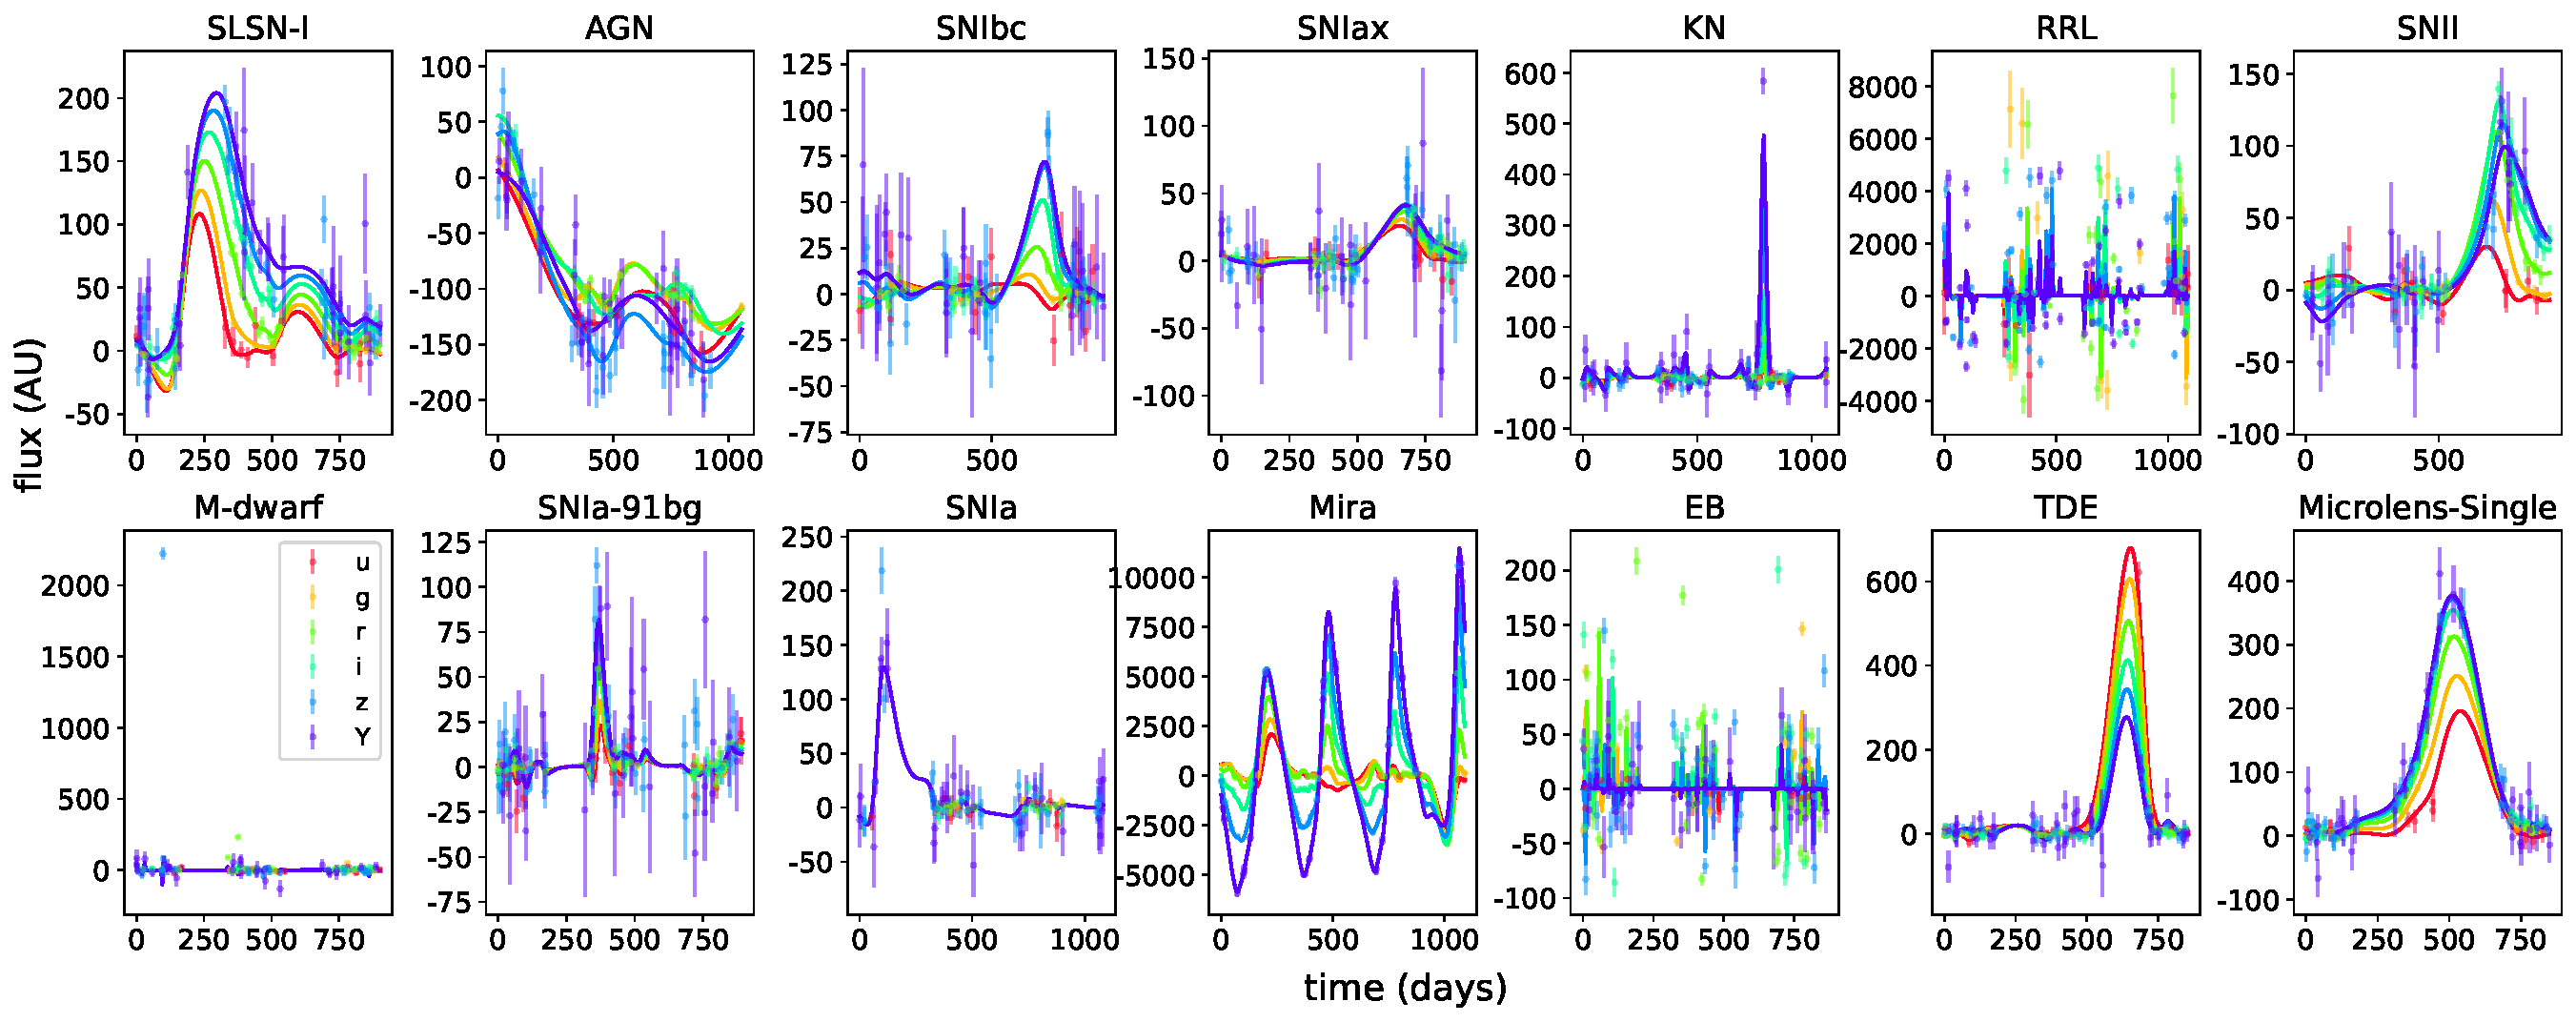
\includegraphics[scale=0.3]{paper/figures/plasticc.pdf}
    \label{fig:plasticc-appendix}
\end{figure}

\paragraph{PLAsTiCC}: We also include simulated light curves from the Photometric LSST Astronomical Time-Series Classification Challenge \citep[PLAsTiCC; ][]{PLAsTiCC_2018}. This diverse dataset contains 14 types of astronomical time-varying objects, simulated using the expected instrument characteristics and survey strategy of the upcoming Legacy Survey of Space and Time \citep[LSST][]{ivezic2019lsst} conducted at the Vera C. Rubin Observatory (Figure~\ref{fig:plasticc-appendix}). It includes two overall categories of time-series objects: \textit{transients}, short-lived events such as supernovae, and \textit{variable} sources, those with fluctuating brightness such as pulsating stars. Specifically, the dataset includes the following transients: type Ia supernovae (SNIa), SNIax, SNIa-91bg, SNIbc, SNII, superluminous supernovae (SLSN), tidal disruption events (TDE), and single lens microlensing events ($\mu$Lens-Single); and the following variable objects: active galactic nuclei (AGN), Mira variables, eclipsing binary systems (EB), and RR Lyrae (RRL); details in Table~\ref{tbl:plasticc-breakdown}.  

\begin{table}[]
    \centering
    \rowcolors{2}{gray!15}{white}
    \resizebox{0.5\textwidth}{!}{
    \begin{tabular}{l c c}
        \toprule
        Object Type & Train Samples & Test Samples \\
        \midrule
        \arrayrulecolor{black!30}
        SNIa & 2,313 & 1,659,831 \\
        SNIa-91bg & 208 & 40,193 \\
        SNIax & 183 & 63,664 \\
        SNII & 1193 & 1,000,150 \\
        SNIbc & 484 & 175,094 \\
        SLSN-I & 175 & 35,782 \\
        TDE & 495 & 13,555 \\
        KN & 102 & 133 \\
        AGN & 370 & 101,424 \\
        RRL & 239 & 197,155 \\
        M-dwarf & 981 & 93,494 \\
        EB & 924 & 96,572 \\
        Mira & 30 & 1,453 \\
        $\mu$-Lens-Single & 151 & 1,303 \\
        \textbf{Total} & \textbf{7,848} & \textbf{3,492,890} \\
        \bottomrule
    \end{tabular}}
    \caption{Breakdown of the PLAsTiCC train and test datasets by object type. The small training set size coupled with the class imbalances make this a challenging classification dataset.}
    \label{tbl:plasticc-breakdown}
\end{table}

Millions of potential new objects are discovered per observing night, and important metadata such as object type, redshift, or other physical parameters, require astronomers to take time-intensive \textit{spectra} of each object. Spectra are a granular brightness vs. wavelength measurement at a single point in time, and are typically only taken for bright, nearby objects which require less exposure time than faint, faraway objects. The vast majority of discovered objects, however, will not have spectra but instead a time series of imaging data taken in 6 broad wavelength ranges, or \textit{photometric bands}. The time-varying behavior of these objects in these coarse wavelength bands does offer important clues about these physical parameters, but expert interpretation of spectra are traditionally required for confident labeling. Thus, our labeled training data comes from the unrepresentative subset of objects with spectra, while the test dataset emulates a sample with photometric time-series data alone.. 

\subsection{Additional Tabular Datasets}

\paragraph{PROVABGS}: The PRObabilistic Value-Added Bright Galaxy Survey (PROVABGS) Catalog \cite{Hahn_2023} will provide posterior measurements of galaxy properties, such as stellar mass ($M_*$), star formation rate ($SFR$), mass-weighted stellar metallicity ($Z_{MW}$), and mass-weighted stellar age ($t_{age,MW}$), for spectra in the DESI Bright Galaxy Survey (BGS). These are inferred using a full Bayesian inference framework and state-of-the-art Spectral Energy Distribution (SED) modeling. At present, as the DESI survey is still on-going, the PROVABGS catalog reports these properties for an early data release (EDR) DESI sample\footnote{\url{https://data.desi.lbl.gov/doc/releases/edr/vac/provabgs/}}, corresponding to roughly 221,000 galaxies, or roughly 1\% of the DESI BGS. For consistency, we use the PROVABGS SED modeling framework to infer the best-fit values of these galaxies properties, and include these as scalars in the PROVABGS dataset. 

\paragraph{Galaxy Zoo}: Galaxy Zoo is a crowdsourcing project recruiting online volunteers to annotate images of galaxies according to visual appearance (e.g. counting spiral arms). These annotations are often aggregated into higher-level classes (e.g. spiral galaxies). \pile includes the Galaxy10 DECaLS dataset\footnote{\href{https://astronn.readthedocs.io/en/latest/galaxy10.html}{https://astronn.readthedocs.io/en/latest/galaxy10.html}}, which aggregates volunteer annotations from GZ DECaLS \cite{Walmsley2023GZDESI} into 10 broad classes and filters to a small (18k) subset of galaxies where the aggregated classes can be confidently assigned. Galaxy10 DECaLS is intended as a benchmark dataset; we provide several baseline models for this benchmark in Sec. \ref{subsec:gz10_baseline}. Unlike the other \pile images, we train our baseline on the RGB images originally bundled with Galaxy10 DECaLS (drawn from the DESI Legacy Survey cutout service) and not the full flux information.



\paragraph{Gaia} \label{par:gaia_astrometry}: The \textit{Gaia} mission, as well as providing optical spectra, is primarily intended for measuring astrometry of stars in the Milky Way. Here we provide astrometric measurements (position on the sky, parallaxes, proper motions, as well as associated uncertainties), photometry, and physical parameters (stellar surface properties like surface gravity and effective temperature) for the subset of stars for which \textit{Gaia} also provides BP/RP spectra, but will later provide measurements for the full 1.46 billion sources catalogued in \textit{Gaia} DR3. Because of the precise position measurements, \textit{Gaia} is a prime candidate for the base on which other (stellar) datasets can be cross-matched.

\section{Additional Details on Baselines}

\subsection{Galaxy10 DECaLS Morphology Classification}
\label{subsec:gz10_baseline}
For the Galaxy10 DECaLS morphology classification baselines, we train all models using an 80/20 train-test split on the GalaxyZoo classification labels and the corresponding Legacy Survey RGB-converted images. We train three canonical computer vision baseline networks - ResNet-18 \citep{he2016deep}, EfficientNetB0 \citep{efficientnet}, and DenseNet121 \citep{huang2017densely} - to classify these images. As they are already range compressed in their conversion to RGB images, we do not apply any range compression. To prevent overfitting, we use data augmentation: random horizontal and vertical flips, random gaussian blurring, random affine translation, and color jittering\footnote{In other astrophysical contexts color jittering tends to be avoided due to its potential to corrupt valuable astrophysical information present in the galaxy colors; however, as we are only concerned with galaxy morphology in this application, we apply it here.}. We train all models using a cross-entropy loss on the training dataset with the Adam optimizer \citep{kingma2014adam}. Training is performed for 10 epochs on a single A100 GPU for each model with a batch size of 128 and a learning rate of $\lambda=10^{-4}$. We report the Top-1 accuracy on the held-out validation test dataset.


\subsection{Physical Property Estimation}
\label{app:physical-property-baselines}
For the physical property inference baselines, we train all models using an 80/20 train-test split on the aforementioned datasets. 

For the image models, we use canonical computer vision baseline networks - ResNet-18 \citep{he2016deep}, EfficientNetB0 \citep{efficientnet}, and DenseNet121 \citep{huang2017densely} - to regress the PROVABGS galaxy properties from the Legacy Survey images. Due to the high dynamic range of the images, we use a range compression scheme to reduce the dynamic range for better optimization. We also use data augmentation - random horizontal and vertical rotations and random gaussian blurring - to reduce overfitting. For the spectrum model, we use a convolutional+attention network with the same architecture as the encoder from the state-of-the-art spectrum encoder from \citep{melchior2023autoencoding}. For the photometry model, we use a simple 5-layer MLP with $d=512$ hidden dimension. Additionally, we $Z$-score the photometry to normalize the data.

We train all models using a mean-squared error (MSE) loss on the training dataset with the Adam optimizer \citep{kingma2014adam}. Training is performed for 25 epochs on a single A100 GPU for each model with a batch size of 256 and a learning rate of $\lambda = 10^{-4}$. We report the $R^2$ performance of all models on the held-out test datasets.

\subsection{PLAsTiCC Photometric Classification and Redshift Estimation}
\label{app:plasticc-baselines}
For the PLAsTiCC baseline model, we use an encoder-only Informer model \citep{zhou2021informer} with 8 encoder layers of 12 attention heads each. The model hidden dimension was chosen to be 768 and the layer MLPs have hidden dimension 256. Due to the 2-dimensional position data (each element of the time-series has an associated time and photometric band/wavelength) and irregular sampling of our dataset, we train a positional encoding based on learnable Fourier features following~\citep{li2021learnable}. We also select a random window of length 300 from each example (and zero-pad examples with fewer than 300 observations) to produce inputs of uniform shape. 
We first pretrain with a masked autoencoding objective:

\begin{align}
\label{eqn:mae_objective}
\sL_{\text{MAE}}(\encoder) = \E_{\inputx\sim \unlabeldist,\inputxp\sim\aug(\cdot \mid \inputx)}[(\encoder(\inputxp)-\inputx)^2]
\end{align}

Here, $\unlabeldist$ is the distribution of unlabeled data that we pretrain with, $\aug$ is the distribution of augmented (masked) inputs, and $\encoder$ is the model. We perform pretraining by randomly masking 60\% of observations of each time-series, a batch size of 256, and learning rate 1e-4 (selected from 1e-3 $\sim$ 1e-6) for 75,000 steps. We finetune the pretrained model with linear probing for 20,000 steps and learning rate 1e-4, then fine-tuning for 10,000 steps at learning rate of 4e-5. The redshift estimation task uses LP learning rate of 5e-4 and FT learning rate of 1e-4. We decrease the learning rate per step with a linear scheduler.

\subsection{YSE Photometric classification}

 We demonstrate an implementation of the \texttt{snmachine} package \citep{lochner2021, alves2022} on the YSE data set with classes mapped to SNe Ia, SNe II, SNe Ib/c, or other.
\texttt{snmachine} offers feature extraction methods based on SN Ia templates \citep{guy2010}, parametric models \citep{newling2012, karpenka2013}, and wavelet analysis \citep{lee2019}, along with wrappers for several classifiers from \texttt{scikit-learn} \citep{pedregosa2011}.
We find that wavelet-based feature extraction combined with the Random Forest classifier, with or without the ensemble AdaBoost classifier, achieves a AUC of 0.90%for the ROC curve 
in SN Ia one-vs-rest classification.


\subsection{Contrastive Image-Spectrum Pretraining}
\label{app:contrastive}

We replicate the results of \texttt{AstroCLIP} method \cite{Parker2024} using the \pile cross-matched DESI and Legacy Surveys. We split the dataset using an 80/20 train-test split We use the same hyperparameter and training suite as in \cite{Parker2024} for training the model on the training suite. We then evaluate model performance by evaluating the zero-shot performance of a $k$-NN algorithm with $k=16$ nearest neighbors on the cross-matched DESI and Legacy Survey and PROVABGS dataset. We report the $R^2$ performance of the model on the held-out test set. Note that the model has never seen the test set during either pretraining or zero-shot ``training''.


\end{document}


